%% ============================================================================
%%  NEUROSHELL COMBINED GROUP DISSERTATION
%%  "NEUROSHELL: AN AUTONOMOUS NATURAL LANGUAGE-DRIVEN ORCHESTRATION FRAMEWORK
%%   FOR OFFENSIVE SECURITY OPERATIONS"
%%  Group R26-CS-018 - Sri Lanka Institute of Information Technology (SLIIT)
%%  Faculty of Computing - Department of Computer Systems Engineering
%%
%%  BUILT ON: the SLIIT undergraduate dissertation template (v1.0)
%%  BUILD:    pdflatex -> biber -> pdflatex x2   (biblatex + biber)
%%  CONFIG:   edit §E USER CONFIGURATION below; then write content in chapters/
%% ============================================================================

%% ============================================================================
%%  §E  USER CONFIGURATION
%% ============================================================================
\documentclass[a4paper,12pt,oneside]{report}

%% --- Candidate list (title page, cover, declaration). One line per student. ---
\newcounter{sliitcand}
\newcommand{\addcandidate}[2]{%
  \stepcounter{sliitcand}%
  \expandafter\gdef\csname sliitcn\arabic{sliitcand}\endcsname{#1}%
  \expandafter\gdef\csname sliitci\arabic{sliitcand}\endcsname{#2}}
\addcandidate{Karunarathna P.M.T.L}{IT22249852}
\addcandidate{Herath H.M.C.H.K}{IT22121592}
\addcandidate{Umayanga H.L.A}{IT22230010}
\addcandidate{Sahan H.P.T}{IT22083678}

%% --- Document metadata -------------------------------------------------------
\newcommand{\DissertationTitle}{NeuroShell: An Autonomous Natural
Language-Driven Orchestration Framework for Offensive Security Operations}
\newcommand{\DissertationSubtitle}{}          % optional
\newcommand{\DegreeFull}{Bachelor of Science (Hons) in Information Technology}
\newcommand{\DegreeShort}{B.Sc. (Hons) Degree in Information Technology}
\newcommand{\Specialization}{Cyber Security}
\newcommand{\DepartmentName}{Department of Computer Systems Engineering}
\newcommand{\InstituteName}{Sri Lanka Institute of Information Technology}
\newcommand{\CountryName}{Sri Lanka}
\newcommand{\SubmissionDate}{October 2026}
\newcommand{\SupervisorName}{Prof. Harinda Fernando}\newcommand{\CoSupervisorName}{Mr. Indunil Daluwatte (Co-Supervisor)}
\newcommand{\CitationStyle}{ieee}              % apa | ieee
\newcommand{\BibResource}{references.bib}

%% --- Switches (true/false) ---------------------------------------------------
\newif\ifHardCover            \HardCoverfalse
\newif\ifIncludeDedication    \IncludeDedicationfalse
\newif\ifIncludeListOfFigures \IncludeListOfFigurestrue
\newif\ifIncludeListOfTables  \IncludeListOfTablestrue
\newif\ifIncludeAbbreviations \IncludeAbbreviationstrue
\newif\ifIncludeAppendices    \IncludeAppendicestrue
\newif\ifIncludeBibliography  \IncludeBibliographyfalse
\newif\ifIncludeGlossary      \IncludeGlossaryfalse
\newif\ifArabicNumberCentered \ArabicNumberCenteredfalse
\newif\ifTocSingleSpaced      \TocSingleSpacedfalse

%% ============================================================================
%%  §F  STANDARDS ENFORCEMENT (preamble + helper macros)
%% ============================================================================

%% --- Fonts: Times New Roman (or closest metric-compatible clone) -------------
\usepackage{iftex}
\ifPDFTeX
  \usepackage[T1]{fontenc}
  \usepackage{amsmath}
  \IfFileExists{newtxtext.sty}{\usepackage{newtxtext,newtxmath}}{\usepackage{mathptmx}}
  \renewcommand{\ttdefault}{pcr}
\else
  \usepackage{amsmath}
  \usepackage{fontspec}
  \IfFontExistsTF{Times New Roman}{\setmainfont{Times New Roman}}{%
    \IfFontExistsTF{Liberation Serif}{\setmainfont{Liberation Serif}}{%
      \IfFontExistsTF{TeX Gyre Termes}{\setmainfont{TeX Gyre Termes}}{%
        \IfFontExistsTF{Nimbus Roman}{\setmainfont{Nimbus Roman}}{}}}}
  \IfFontExistsTF{Courier New}{\setmonofont{Courier New}}{%
    \IfFontExistsTF{Liberation Mono}{\setmonofont{Liberation Mono}}{%
      \IfFontExistsTF{TeX Gyre Cursor}{\setmonofont{TeX Gyre Cursor}}{}}}
\fi
\usepackage{microtype}

%% --- Page geometry -----------------------------------------------------------
\usepackage[a4paper,left=40mm,right=25mm,top=25mm,bottom=40mm,
            headheight=14.5pt,headsep=5mm,footskip=15mm]{geometry}

%% --- Helper packages ---------------------------------------------------------
\usepackage{etoolbox}
\usepackage{setspace}
\usepackage{graphicx}
\usepackage{xcolor}
\usepackage{array}
\usepackage{longtable}
\usepackage{booktabs}
\usepackage{enumitem}
\usepackage{csquotes}
\usepackage{pagecolor}
\definecolor{sliitgold}{RGB}{212,175,55}

%% --- Line spacing + paragraphs ------------------------------------------------
\onehalfspacing
\setlength{\parindent}{0pt}
\setlength{\parskip}{6pt plus 1pt}
\clubpenalty=10000 \widowpenalty=10000
\setlist{topsep=3pt,itemsep=0pt,parsep=0pt}
\renewenvironment{quote}{\list{}{\leftmargin=10mm\rightmargin=10mm}\item\relax\singlespacing}{\endlist}
\AtBeginEnvironment{quotation}{\singlespacing}

%% --- Heading numbering depth ---------------------------------------------------
\setcounter{secnumdepth}{2}
\setcounter{tocdepth}{2}

%% --- Headings: chapter ALL CAPS 14 pt bold; section/sub-section 12 pt bold ----
\usepackage{titlesec}
\newcommand{\sliitheadalign}{\raggedright}
\newcommand{\sliitUC}[1]{\MakeUppercase{#1}}
\newcommand{\sliitchapfont}{\bfseries\fontsize{14}{16.8}\selectfont}
\newcommand{\sliitsecfont}{\bfseries\fontsize{12}{14.4}\selectfont}
\newcommand{\sliitchaplabel}{\thechapter.}
\makeatletter
\def\@makechapterhead#1{{\parindent\z@\sliitheadalign\sliitchapfont
  \sliitchaplabel\hspace{0.6em}\sliitUC{#1}\par\nobreak\vskip 24\p@}}
\def\@makeschapterhead#1{{\parindent\z@\sliitheadalign\sliitchapfont
  \sliitUC{#1}\par\nobreak\vskip 24\p@}}
\makeatother
\titleformat{\section}{\sliitheadalign\sliitsecfont}{\thesection}{0.6em}{}
\titleformat{\subsection}{\sliitheadalign\sliitsecfont}{\thesubsection}{0.6em}{}
\titleformat{\subsubsection}{\sliitheadalign\sliitsecfont\itshape}{\thesubsubsection}{0.6em}{}
\titlespacing*{\section}{0pt}{18pt plus 2pt minus 2pt}{6pt}
\titlespacing*{\subsection}{0pt}{12pt plus 2pt minus 2pt}{4pt}
\titlespacing*{\subsubsection}{0pt}{12pt plus 2pt minus 2pt}{4pt}

%% --- Contents / lists layout --------------------------------------------------
\usepackage{tocloft}
\renewcommand{\cftdotsep}{2}
\renewcommand{\cftchapfont}{\normalfont}
\renewcommand{\cftchappagefont}{\normalfont}
\renewcommand{\cftchapleader}{\cftdotfill{\cftdotsep}}
\renewcommand{\cftchapaftersnum}{.}
\setlength{\cftbeforechapskip}{0pt}
\setlength{\cftbeforesecskip}{0pt}
\setlength{\cftbeforesubsecskip}{0pt}
\setlength{\cftchapindent}{0pt}   \setlength{\cftchapnumwidth}{2em}
\setlength{\cftsecindent}{2em}    \setlength{\cftsecnumwidth}{2.5em}
\setlength{\cftsubsecindent}{4.5em}\setlength{\cftsubsecnumwidth}{3.2em}
\renewcommand{\cftfigpresnum}{Figure~}  \setlength{\cftfigindent}{0pt}\setlength{\cftfignumwidth}{5.5em}
\renewcommand{\cfttabpresnum}{Table~}   \setlength{\cfttabindent}{0pt}\setlength{\cfttabnumwidth}{5em}
\setlength{\cftbeforefigskip}{0pt}
\setlength{\cftbeforetabskip}{0pt}

%% --- Page numbering / footers ---------------------------------------------------
\usepackage{fancyhdr}
\newcommand{\sliitsetfooter}[1]{%
  \fancypagestyle{plain}{\fancyhf{}\fancyfoot[#1]{\thepage}%
    \renewcommand{\headrulewidth}{0pt}\renewcommand{\footrulewidth}{0pt}}%
  \fancypagestyle{sliit}{\fancyhf{}\fancyfoot[#1]{\thepage}%
    \renewcommand{\headrulewidth}{0pt}\renewcommand{\footrulewidth}{0pt}}%
  \pagestyle{sliit}}
\newcommand{\sliitsetbodyfooter}{%
  \ifArabicNumberCentered\sliitsetfooter{C}\else\sliitsetfooter{R}\fi}
\newcommand{\sliitstartbody}{\clearpage\pagenumbering{arabic}\sliitsetbodyfooter}

%% --- Captions, floats, tables ---------------------------------------------------
\usepackage{caption}
\captionsetup{labelsep=colon,justification=centering,font={normalsize,singlespacing}}
\captionsetup[figure]{position=bottom,skip=8pt}
\captionsetup[table]{position=top,skip=6pt}
\newcommand{\sliittablestyle}{\singlespacing\small\renewcommand{\arraystretch}{1.25}\selectfont}
\AtBeginEnvironment{figure}{\centering}
\AtBeginEnvironment{table}{\centering\sliittablestyle}
\AtBeginEnvironment{longtable}{\singlespacing\renewcommand{\arraystretch}{1.25}\selectfont}
\setlength{\LTpre}{4pt}\setlength{\LTpost}{4pt}
\newcommand{\sliitsource}[1]{\par\vspace{3pt}{\centering\singlespacing\small\textit{Source:} #1\par}}
\newcommand{\OriginalInColor}{(Original in Color)}

%% --- Bibliography: APA or IEEE via biblatex/biber ------------------------------
\ifdefstring{\CitationStyle}{ieee}
  {\usepackage[backend=biber,style=ieee,defernumbers=true]{biblatex}}
  {\usepackage[backend=biber,style=apa,defernumbers=true]{biblatex}}

%% --- Hyperlinks + cross references ----------------------------------------------
\usepackage[hidelinks,bookmarksnumbered,pdfpagelabels=true,plainpages=false]{hyperref}
\AtBeginDocument{\hypersetup{pdftitle={\DissertationTitle},pdfauthor={\csname sliitcn1\endcsname}}}
\usepackage[capitalise,noabbrev]{cleveref}
\crefname{figure}{Figure}{Figures}\Crefname{figure}{Figure}{Figures}
\crefname{table}{Table}{Tables}\Crefname{table}{Table}{Tables}
\crefname{chapter}{Chapter}{Chapters}\Crefname{chapter}{Chapter}{Chapters}
\crefname{section}{Section}{Sections}\Crefname{section}{Section}{Sections}
\crefname{appendix}{Appendix}{Appendices}\Crefname{appendix}{Appendix}{Appendices}

%% --- Helper macros ----------------------------------------------------------------
\newcommand{\TODO}[1]{\textbf{[TODO: #1]}\PackageWarning{sliit}{TODO: #1}}
\newlength{\sliitline}\setlength{\sliitline}{24pt}
\newlength{\sliittopgap}

\newcounter{sliitcandi}
\newcommand{\sliitforcands}[1]{%
  \setcounter{sliitcandi}{0}%
  \whileboolexpr{test{\ifnumcomp{\value{sliitcandi}}{<}{\value{sliitcand}}}}{%
    \stepcounter{sliitcandi}%
    \expandafter\let\expandafter\sliitcn\csname sliitcn\arabic{sliitcandi}\endcsname
    \expandafter\let\expandafter\sliitci\csname sliitci\arabic{sliitcandi}\endcsname
    #1}}

\newcommand{\sliitprelimchapter}[1]{%
  \chapter*{#1}\phantomsection\addcontentsline{toc}{chapter}{#1}}

\newcommand{\sliitcomputetopgap}{%
  \setlength{\sliittopgap}{8\sliitline}%
  \sliitforcands{\addtolength{\sliittopgap}{-2\sliitline}}%
  \ifdim\sliittopgap<0pt \setlength{\sliittopgap}{0pt}\fi}

%% --- Cover page (hard-bound final copy only) -------------------------------------
\newcommand{\sliitmakecover}{%
  \begingroup\sliitcomputetopgap
  \pagecolor{black}\color{sliitgold}%
  \thispagestyle{empty}\centering\singlespacing\setlength{\parskip}{0pt}
  \vbox to \dimexpr 9in-25mm\relax{%
    \vskip\sliittopgap
    {\bfseries\fontsize{16}{24}\selectfont\MakeUppercase{\DissertationTitle}\par}%
    \vskip 1\sliitline
    \sliitforcands{{\fontsize{14}{21}\selectfont\sliitcn\par}{\fontsize{14}{21}\selectfont(\sliitci)\par}}%
    \vskip 2\sliitline
    {\fontsize{14}{21}\selectfont \DegreeShort\par Specializing in \Specialization\par
     \DepartmentName\par \InstituteName\par \CountryName\par}%
    \vss}%
  {\fontsize{14}{21}\selectfont\SubmissionDate\par}%
  \clearpage
  \endgroup
  \nopagecolor}

%% --- Title page ---------------------------------------------------------------------
\newcommand{\sliitmaketitlepage}{%
  \begingroup\sliitcomputetopgap
  \thispagestyle{empty}\centering\singlespacing\setlength{\parskip}{0pt}
  \vspace*{\sliittopgap}%
  {\bfseries\fontsize{16}{24}\selectfont\MakeUppercase{\DissertationTitle}\par}%
  \ifdefempty{\DissertationSubtitle}{}{\vskip .5\sliitline
    {\bfseries\fontsize{14}{21}\selectfont\DissertationSubtitle\par}}%
  \vskip 1\sliitline
  \sliitforcands{{\fontsize{14}{21}\selectfont\sliitcn\par}{\fontsize{14}{21}\selectfont(\sliitci)\par}}%
  \vskip 2\sliitline
  {\fontsize{12}{18}\selectfont Dissertation submitted in partial fulfillment of the requirements\\
   for the \DegreeFull\par}%
  \vskip 2\sliitline
  {\fontsize{14}{21}\selectfont \DepartmentName\par \InstituteName\par \CountryName\par}%
  \vskip 1\sliitline
  {\fontsize{14}{21}\selectfont\SubmissionDate\par}%
  \clearpage
  \endgroup}

%% --- Declaration page -----------------------------------------------------------------
\newcommand{\sliitdeclaration}{%
  \sliitprelimchapter{Declaration of the Candidates \& Supervisors}%
  We declare that this is our own work and this dissertation does not incorporate without
  acknowledgement any material previously submitted for a Degree or Diploma in any other
  University or institute of higher learning and to the best of our knowledge and belief it
  does not contain any material previously published or written by another person except
  where the acknowledgement is made in the text.

  Also, we hereby grant to \InstituteName, the nonexclusive right to reproduce and distribute
  this dissertation, in whole or in part in print, electronic or other medium. We retain the
  right to use this content in whole or part in future works (such as articles or books).

  \begingroup\singlespacing\vspace{6pt}%
  \sliitforcands{%
    \noindent\textbf{\sliitcn} (\sliitci)\par\vspace{14pt}
    \noindent Signature:\ \underline{\hspace{6cm}}\hfill Date:\ \underline{\hspace{3.5cm}}\par
    \vspace{12pt}}%
  \endgroup

  \vspace{1\sliitline}
  \textbf{Statement of the supervisor}

  The above \ifnum\value{sliitcand}>1 candidates have\else candidate has\fi\ carried out
  research for the bachelor's degree dissertation under my supervision.

  \begingroup\singlespacing\vspace{14pt}%
  \noindent Signature of the supervisor:\ \underline{\hspace{5cm}}\hfill Date:\ \underline{\hspace{3.5cm}}\par
  \noindent\SupervisorName\par
  \noindent\CoSupervisorName\par
  \endgroup}

%% --- Dedication (optional) -------------------------------------------------------------
\newcommand{\sliitdedication}[1]{%
  \sliitprelimchapter{Dedication}\vspace*{\fill}\begin{center}\textit{#1}\end{center}\vspace*{\fill}}

%% --- Abstract --------------------------------------------------------------------------
\newenvironment{sliitabstract}
  {\clearpage\phantomsection\addcontentsline{toc}{chapter}{Abstract}%
   {\sliitheadalign\bfseries\fontsize{12}{14.4}\selectfont Abstract\par}\vspace{12pt}%
   \begingroup\singlespacing\fontsize{11}{13.2}\selectfont}
  {\par\endgroup\clearpage}
\newcommand{\sliitkeywords}[1]{\par\vspace{6pt}\noindent\textbf{Keywords:} #1\par}

%% --- Table of contents + lists -----------------------------------------------------------
\makeatletter
\newcommand{\sliittocspacing}{\ifTocSingleSpaced\singlespacing\fi}
\newcommand{\sliittoc}{%
  \clearpage\phantomsection\addcontentsline{toc}{chapter}{Table of Contents}%
  \chapter*{Table of Contents}%
  \begingroup\sliittocspacing\@starttoc{toc}\endgroup}
\newcommand{\sliitlistoffigures}{%
  \clearpage\phantomsection\addcontentsline{toc}{chapter}{List of Figures}%
  \chapter*{List of Figures}{\noindent\hfill\textbf{Page}\par}%
  \begingroup\sliittocspacing\@starttoc{lof}\endgroup}
\newcommand{\sliitlistoftables}{%
  \clearpage\phantomsection\addcontentsline{toc}{chapter}{List of Tables}%
  \chapter*{List of Tables}{\noindent\hfill\textbf{Page}\par}%
  \begingroup\sliittocspacing\@starttoc{lot}\endgroup}
\newcommand{\l@appendix}{\@dottedtocline{1}{0em}{7.5em}}
\newcommand{\sliitlistofappendices}{%
  \clearpage\phantomsection\addcontentsline{toc}{chapter}{List of Appendices}%
  \chapter*{List of Appendices}%
  {\noindent\makebox[7.5em][l]{\bfseries Appendix}\bfseries Description\hfill\bfseries Page\par}%
  \begingroup\sliittocspacing\@starttoc{loa}\endgroup}
\makeatother

%% --- Abbreviations / glossary helpers -----------------------------------------------------
\newcommand{\abbrevrow}[2]{#1 & #2\\[3pt]}
\newcommand{\glossentry}[2]{\noindent\textbf{#1} --- #2\par}

%% --- Appendices ---------------------------------------------------------------------------
\newcommand{\sliitbeginappendices}{%
  \clearpage
  \appendix
  \renewcommand{\sliitchaplabel}{\MakeUppercase{Appendix}~\thechapter:}%
  \addtocontents{toc}{\protect\renewcommand{\protect\cftchappresnum}{Appendix~}%
    \protect\renewcommand{\protect\cftchapaftersnum}{:}%
    \protect\setlength{\protect\cftchapnumwidth}{6.5em}}}
\newcommand{\sliitappendix}[1]{%
  \chapter{#1}\addcontentsline{loa}{appendix}{\protect\numberline{Appendix \thechapter}#1}}

%% --- Reference list ------------------------------------------------------------------------
\defbibheading{sliitbib}{\clearpage\phantomsection\addcontentsline{toc}{chapter}{Reference List}%
  \chapter*{Reference List}}
\defbibheading{sliitbibliography}{\clearpage\phantomsection\addcontentsline{toc}{chapter}{Bibliography}%
  \chapter*{Bibliography}}
\newcommand{\sliitprintreferences}{%
  \begingroup\singlespacing\selectfont\setlength{\bibitemsep}{\baselineskip}%
  \printbibliography[heading=sliitbib,notkeyword=bibliographyonly]%
  \endgroup}
\newcommand{\sliitprintbibliography}{%
  \begingroup\singlespacing\selectfont\setlength{\bibitemsep}{\baselineskip}%
  \nocite{*}\printbibliography[heading=sliitbibliography,keyword=bibliographyonly]%
  \endgroup}

\addbibresource{\BibResource}

%% Figures: component media folders are referenced in place (relative paths).
%% C-01 <C-01-Intetrecodnition Engine.pdf/vertopal_433ccb30063e47f1ba4c32a79683aeea/media>
%% C-02 <C-02-Dynamic planner and rag enginee/vertopal_80eb40840323498cb949d017d9b2b63a/media>
%% C-03 <C-03-Adoptive executer and error Recovery engine/vertopal_05e97fad080746c9b767567e93f99da6/media>
%% C-04 <C-04-AI-Driven Vulnerability Analysis Engine/vertopal_0d07bf200b61446895bb385b0aa02c6b/media>

%% ============================================================================
%%  §G  DOCUMENT BODY
%% ============================================================================
\begin{document}

%% ---- Cover (hard copy) + Title page -----------------------------------------
\pagenumbering{gobble}\pagestyle{empty}
\ifHardCover\sliitmakecover\fi
\sliitmaketitlepage

%% ---- Preliminary pages: i, ii, iii ... centred at bottom ---------------------
\pagenumbering{roman}\sliitsetfooter{C}

\sliitdeclaration

\ifIncludeDedication
  \sliitdedication{To our families and to the security community.}
\fi

\begin{sliitabstract}
  Automated security assessments require an analyst to translate a natural-language
request into tool commands, run those commands, interpret their output, and
recover when a tool fails. Each step is manual, error-prone, and difficult to
automate end-to-end because an error message in the middle of a scan normally
stops the whole operation. This dissertation presents NeuroShell, an autonomous,
natural-language-driven orchestration framework for offensive security
operations that addresses this gap with four cooperating components.

The Intent Recognition Engine (Component 1) converts free-form security requests
into validated, machine-readable intent contracts. A small, offline, CPU-only
language model acts as a guarded natural-language gateway: a multi-stage
pipeline and deterministic validation stack reject malformed, out-of-scope and
adversarial outputs before any downstream action. The Dynamic Planner and
Retrieval-Augmented Generation Engine (Component 2) translates a structured
intent into a tool command for Nmap, Nikto or Gobuster, using retrieval over a
documentation knowledge base to ground command synthesis, and applies explicit
validation and safety checks. The Adaptive Execution and Error-Recovery Engine
(Component 3) runs every command in a locked-down Docker sandbox, and when a
command fails it labels the error, plans a fix with a local AI model, and retries
automatically, while refusing any command that fails its safety checks. The
AI-Driven Vulnerability Analysis Engine (Component 4) parses the execution
records produced by the security tools, enriches findings with CISA KEV, EPSS
and NVD intelligence, and prioritises vulnerabilities with an XGBoost-based
classifier explained by SHAP values.

NeuroShell keeps model inference entirely on the local machine, so no command,
error text or target ever leaves the deployment boundary. Evaluations measured
command-intent accuracy at 87.54\% for the planner, error-labelling macro-F1 of
99.1\% (and above 96\% under heavy message noise) for the recovery engine, and a
curated vulnerability-classification pipeline with strong discriminative
performance on a 155,852-record data set. Findings confirm that deterministic
validation, documentation grounding, sandboxed recovery and explainable
vulnerability scoring each contribute to a safer automated workflow. The
framework narrows the gap left by current AI copilots, which stop at tool
selection, execute without an autonomous error-recovery loop, or rely on
cloud-hosted models that conflict with strict data-governance requirements.

\sliitkeywords{Offensive Security, Natural Language Orchestration, Intent
Recognition, Retrieval-Augmented Generation, Error Recovery, Vulnerability
Analysis, Offline Language Models}
\end{sliitabstract}

\sliitprelimchapter{Acknowledgement}
We wish to express our deepest gratitude to our principal supervisor, Prof.
Harinda Fernando, and our co-supervisor, Mr. Indunil Daluwatte, for their
invaluable guidance, steady support and constructive feedback throughout this
research. Their expertise and encouragement shaped the direction, development
and quality of this work, and each individual component of the NeuroShell
framework.

We are also sincerely grateful to the academic staff of the Faculty of Computing
at the Sri Lanka Institute of Information Technology (SLIIT) for the knowledge,
the supportive learning environment and the resources that made research in
cybersecurity possible. The questionnaires, evaluation instruments and lab
facilities provided by the department supported every phase of this project.

Our special thanks go to the members of Research Group R26-CS-018 for their
cooperation, their technical discussions and the spirit of collaboration in
which we built the NeuroShell framework together. Integrating four individually
developed components into a single orchestration chain demanded sustained
communication about interface contracts, data formats and shared state, and this
work would not have been possible without that collective effort.

Finally, we thank our families and friends from the bottom of our hearts for
their patience, encouragement and moral support throughout our B.Sc. (Hons)
degree programme and the completion of this research project.

\sliittoc
\ifIncludeListOfFigures\sliitlistoffigures\fi
\ifIncludeListOfTables\sliitlistoftables\fi

\ifIncludeAbbreviations
  \sliitprelimchapter{List of Abbreviations}
  \begin{longtable}{@{}p{0.26\textwidth}p{0.70\textwidth}@{}}
  \textbf{Abbreviation} & \textbf{Description}\\[3pt]
  \abbrevrow{AEERE}{Adaptive Execution and Error-Recovery Engine}
  \abbrevrow{AI}{Artificial Intelligence}
  \abbrevrow{API}{Application Programming Interface}
  \abbrevrow{AVAE}{AI-Driven Vulnerability Analysis Engine}
  \abbrevrow{AUC}{Area Under the Curve}
  \abbrevrow{CISA}{Cybersecurity and Infrastructure Security Agency}
  \abbrevrow{CPU}{Central Processing Unit}
  \abbrevrow{CVE}{Common Vulnerabilities and Exposures}
  \abbrevrow{CVSS}{Common Vulnerability Scoring System}
  \abbrevrow{DSR}{Design Science Research}
  \abbrevrow{EPSS}{Exploit Prediction Scoring System}
  \abbrevrow{F1}{Harmonic mean of precision and recall}
  \abbrevrow{FastAPI}{Python asynchronous web framework used for component APIs}
  \abbrevrow{GGUF}{GPT-Generated Unified Format (quantised model format)}
  \abbrevrow{HTTP}{Hypertext Transfer Protocol}
  \abbrevrow{IRE}{Intent Recognition Engine}
  \abbrevrow{JSON}{JavaScript Object Notation}
  \abbrevrow{KEV}{Known Exploited Vulnerabilities}
  \abbrevrow{KV}{Kali Virtual environment container}
  \abbrevrow{LLM}{Large Language Model}
  \abbrevrow{LoRA}{Low-Rank Adaptation}
  \abbrevrow{ML}{Machine Learning}
  \abbrevrow{NLU}{Natural Language Understanding}
  \abbrevrow{NVD}{National Vulnerability Database}
  \abbrevrow{Ollama}{Local LLM inference runtime}
  \abbrevrow{PR-AUC}{Precision--Recall Area Under the Curve}
  \abbrevrow{Q8\_0}{8-bit quantisation format for GGUF models}
  \abbrevrow{RAG}{Retrieval-Augmented Generation}
  \abbrevrow{RBAC}{Role-Based Access Control}
  \abbrevrow{ROC-AUC}{Receiver Operating Characteristic Area Under the Curve}
  \abbrevrow{RQ}{Research Question}
  \abbrevrow{SHAP}{SHapley Additive exPlanations}
  \abbrevrow{SDG}{Sustainable Development Goal}
  \abbrevrow{SQLite}{Self-contained SQL database engine}
  \abbrevrow{SSG}{Supplementary Self-Consistency Gate}
  \abbrevrow{TF-IDF}{Term Frequency--Inverse Document Frequency}
  \abbrevrow{XGBoost}{Extreme Gradient Boosting}
\end{longtable}
\fi

\ifIncludeAppendices\sliitlistofappendices\fi

%% ---- Body: Arabic numerals restart at 1 -------------------------------------
\sliitstartbody

\chapter{Introduction}\label{ch:introduction}

\section{Background and Literature Survey}\label{sec:background}

\subsection{Overall Project Context: The NeuroShell Framework}\label{sec:ctx-overall}

A cybersecurity assessment involves more than selecting a tool and running a
command. The analyst must identify the intended operation, specify the correct
target, select suitable options, interpret the resulting output, and recover
when a tool fails. NeuroShell brings these activities into a modular workflow in
which each component has a defined responsibility. The framework is intended to
support authorised security assessments while preserving the information needed
to move from a user's request to an operational action, and finally to an
explainable vulnerability report.

The process begins with a natural-language request submitted through the user
interface. The Intent Recognition Engine (IRE, Component~1) interprets the
request and produces a structured representation of the task. This
representation carries operational information such as the intent, target,
ports, and modifiers to the planning component. The Dynamic Planner and
Retrieval-Augmented Generation Engine (Component~2) turns that structured task
into a validated command grounded in tool documentation. The Adaptive Execution
and Error-Recovery Engine (Component~3) runs the command inside a locked-down
container, captures the output, and fixes failures on its own. Finally, the
AI-Driven Vulnerability Analysis Engine (Component~4) takes the execution logs,
extracts security findings, and produces prioritised, explainable vulnerability
information. \cref{fig:fourchain} shows the complete component chain and the
data flow that connects the four engines.

\begin{figure}[htbp]
  \centering
  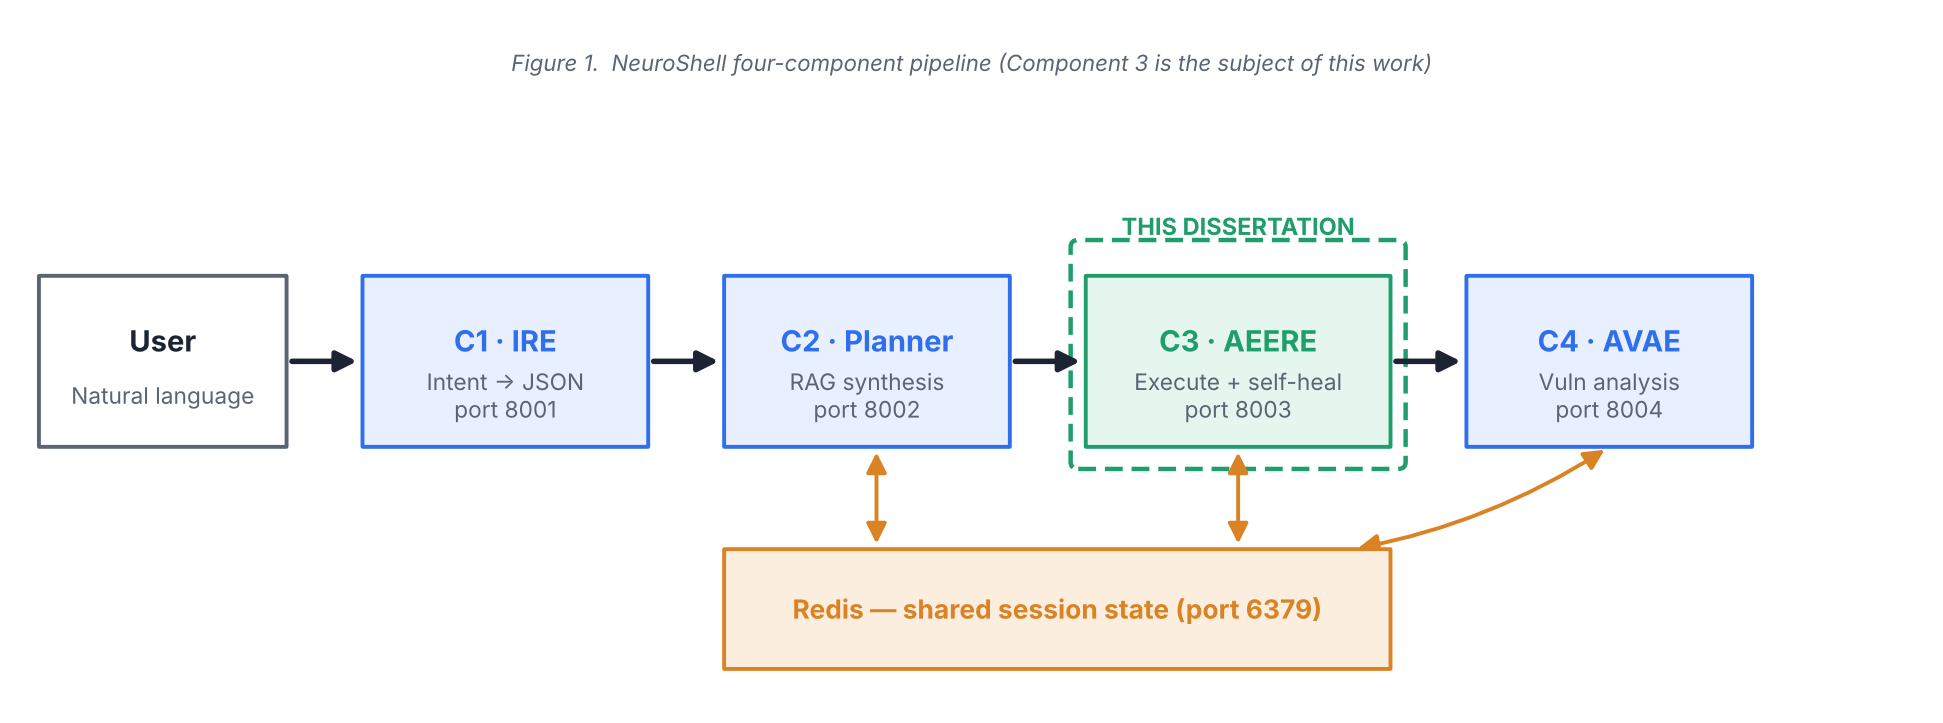
\includegraphics[width=0.92\textwidth]{C-03-Adoptive executer and error Recovery engine/vertopal_05e97fad080746c9b767567e93f99da6/media/image1.png}
  \caption{The four parts of NeuroShell (Component 3, the AEERE, is the subject
  of one of the component reports).}\label{fig:fourchain}
\end{figure}

The framework is organised as a group project (R26-CS-018) in which four
students each designed, implemented, and evaluated one component. The components
communicate over HTTP through FastAPI endpoints (ports 8001--8004) and share
state through Redis, so that each stage receives a well-defined structured
payload and produces a structured result. Separating the stages gives each
component an explicit input contract and provides a basis for checking whether
the information produced by one stage is preserved by the next.

\subsection{The Intent Recognition Engine (Component 1)}\label{sec:ctx-ire}

The IRE addresses the first gap in the chain: translating a free-form security
request into a validated, machine-readable intent contract. Large language
models (LLMs) are increasingly used to translate natural-language security
requests into machine-executable actions, but their stochastic output can
contain malformed structures, hallucinated parameters, out-of-scope targets, and
adversarial content, creating safety risks when connected to automated security
tools~\cite{deng2024pentestgpt}.

The IRE combines an offline, CPU-based language model with a multi-stage
pipeline and deterministic validation. The design constrains the raw output of
the model before any downstream dispatch: a guarded natural-language-understanding
gateway that accepts schema-valid, authorised, and in-scope intent contracts only.
The engine supports four security tools (Nmap, Gobuster, Nikto, and Nuclei) across
nine intent classes and is evaluated on 1,500 records with two offline backends
(Gemma and Qwen). Its closed trust boundary means no request text leaves the
device at inference time~\cite{liu2023promptinjection,nistairmf2023}.

\subsection{The Dynamic Planner and RAG Engine (Component 2)}\label{sec:ctx-planner}

Recognising a task does not, by itself, establish how that task should be
performed. The Dynamic Planner and Retrieval-Augmented Generation Engine
(Component~2) addresses the transition from a structured cybersecurity task to a
command-line instruction: it must select a suitable tool, preserve the supplied
target and operational parameters, and express the requested behaviour using the
syntax supported by that tool.

The component combines structured intent processing with retrieval of relevant
tool documentation. The knowledge base contains documentation and usage
information for the supported tools (Nmap, Nikto, and Gobuster). During planning,
relevant passages are retrieved and supplied as context for command synthesis,
so the generation stage has an explicit reference for tool options and usage
while the documentation collection is maintained separately from the language
model. Command correctness is treated as having several dimensions: a command may
use valid syntax while performing a different operation, or it may reflect the
intended operation while containing an unsupported argument. Evaluating syntax
alone therefore provides an incomplete assessment of the planner's
reliability~\cite{lewis2020rag,reimers2019sentencebert}.

\subsection{The Adaptive Execution and Error-Recovery Engine (Component 3)}\label{sec:ctx-aeere}

Security testers use a long list of command-line tools on Kali Linux, and these
tools fail very often: a tool may not be installed, a permission may be missing,
a target may be unreachable, or a command may use a wrong flag. When this
happens, conventional automated scans simply stop and wait. Even newer AI tools
such as PentestGPT, VulnBot, and xOffense do the same thing: they show the error
to the user and give up~\cite{pentestgpt,deng2024pentestgpt,vulnbot2025,xoffense2025}.

The Adaptive Execution and Error-Recovery Engine (AEERE, Component~3) addresses
this failure. Every command runs inside a Docker container with Kali Linux, so
nothing can harm the real computer. If the command fails, the engine reads the
error, works out what went wrong, fixes the command, and tries again, all by
itself. To work out what went wrong, it uses three steps one after another: a
fast pattern check, a text-similarity check, and finally a local AI model (Gemma,
run through Ollama) that reasons about the error. Before any fixed command is
allowed to run, it must pass three safety checks. Because the AI runs on the
same computer, no command, error, or target is ever sent to the
internet~\cite{yao2023react,shinn2023reflexion,gou2024critic}.

\subsection{The AI-Driven Vulnerability Analysis Engine (Component 4)}\label{sec:ctx-avae}

Automated security tools generate extensive vulnerability information that
needs manual interpretation and prioritisation. Traditional severity-based
approaches, particularly the Common Vulnerability Scoring System (CVSS), do not
by themselves establish whether a vulnerability has been exploited in the
real world. The AI-Driven Vulnerability Analysis Engine (AVAE, Component~4) is
responsible for transforming raw security assessment outputs into structured and
prioritised vulnerability information.

The component receives execution results from the AEERE through a structured
JSON interface and processes outputs of Nmap, Nikto, and Gobuster using dedicated
parsing mechanisms. It extracts IP addresses, open ports, running services, CVE
identifiers, and discovered web paths, and enriches them with vulnerability
intelligence from the National Vulnerability Database (NVD), the CISA Known
Exploited Vulnerabilities (KEV) catalogue, and the Exploit Prediction Scoring
System (EPSS). A central contribution is an Extreme Gradient Boosting (XGBoost)
classifier that uses five features (CVSS v3 score, EPSS score, EPSS percentile,
vulnerability age, and an engineered CVSS--EPSS interaction) to identify
vulnerabilities associated with documented exploitation evidence, with SHapley
Additive exPlanations (SHAP) providing interpretability. Neo4j graph-based
storage maintains relationships between sessions, hosts, services, and
vulnerabilities~\cite{bozorgi2010beyond,sabottke2015vulnerability,lundberg2017shap,
chen2016xgboost,jacobs2023epss}.

\subsection{Comparison with Existing Systems}\label{sec:existing}

Research on LLMs in penetration testing has demonstrated their potential to
support tool use, interpret execution output, and propose subsequent actions.
PentestGPT investigates these capabilities within a broader penetration-testing
workflow and identifies difficulties in maintaining the context of an entire
testing scenario~\cite{deng2024pentestgpt}; it relies on cloud-hosted GPT-class
models and offers no autonomous error-recovery loop. ReAct and Reflexion
demonstrate reasoning-acting and verbal self-reflection patterns for agents, and
CRITIC implements tool-interactive self-correction, but none of these is
specialised for security-tool failure recovery or operates fully
offline~\cite{yao2023react,shinn2023reflexion,gou2024critic}. AutoAttacker,
VulnBot, and xOffense move closer to autonomous offensive operations, yet they
depend on remote models and still stop on tool
failure~\cite{autoattacker2024,vulnbot2025,xoffense2025}. RepairAgent and SCoRe
target program repair rather than penetration-testing tool chains
~\cite{repairagent2024,score2024}. NL2Bash and related work show that
natural-language-to-shell translation is feasible but do not integrate intent
guarding, sandboxed execution, or vulnerability analysis~\cite{nl2bash2018}.

The NeuroShell framework differs from each of these categories in at least one
respect. Unlike generation-side copilots, it guards every intent with
deterministic validation. Unlike tool-integration work, it grounds command
synthesis in a maintainable documentation knowledge base. Unlike execution
frameworks that stop on failure, it autonomously recovers tool errors inside a
sandbox. And unlike cloud-hosted analysis pipelines, it runs all model inference
locally, which is a structural difference for air-gapped and regulated
deployments. \cref{tab:existing-chart} summarises this positioning.

\begin{table}[htbp]
  \centering
  \begin{tabular}{@{}p{0.26\textwidth}p{0.70\textwidth}@{}}
    \toprule
    \textbf{Category} & \textbf{Limitation addressed by NeuroShell}\\
    \midrule
    Deterministic tooling (Nmap, Metasploit) & No natural-language interface; no analysis of intent safety.\\
    Generation-side copilots (PentestGPT) & No deterministic intent guarding; cloud-hosted; no error recovery.\\
    Tool-integration techniques (ReAct, CRITIC) & Not security-specific; no sandboxed execution chain.\\
    Autonomous offensive agents (VulnBot, xOffense) & Stop on tool failure; remote models; no vulnerability prioritisation.\\
    Repair/self-correction (RepairAgent, SCoRe) & Target program repair, not security-tool failure recovery.\\
    \bottomrule
  \end{tabular}
  \caption{Positioning of NeuroShell against existing system categories.}\label{tab:existing-chart}
\end{table}

\subsection{Conceptual Framework and Design Principles}\label{sec:conceptual}

The combined design rests on a small set of principles that recur in every
component. First, \emph{boundary over intent}: the framework prefers to state,
enforce, and verify its boundaries (schema, scope, authorisation, sandbox)
rather than to rely on the model's good behaviour. Second, \emph{structured
contracts}: each stage communicates through a validated, machine-readable
payload (intent contract, planner output, execution result, analysis output)
rather than prose. Third, \emph{guarded autonomy}: the framework automates the
intent-to-command-to-report chain, but every automatically generated artefact
must pass a deterministic predicate before it is used. Fourth, \emph{closed
trust boundary}: all model inference is local, and no operational text leaves
the deployment machine.

\begin{figure}[htbp]
  \centering
  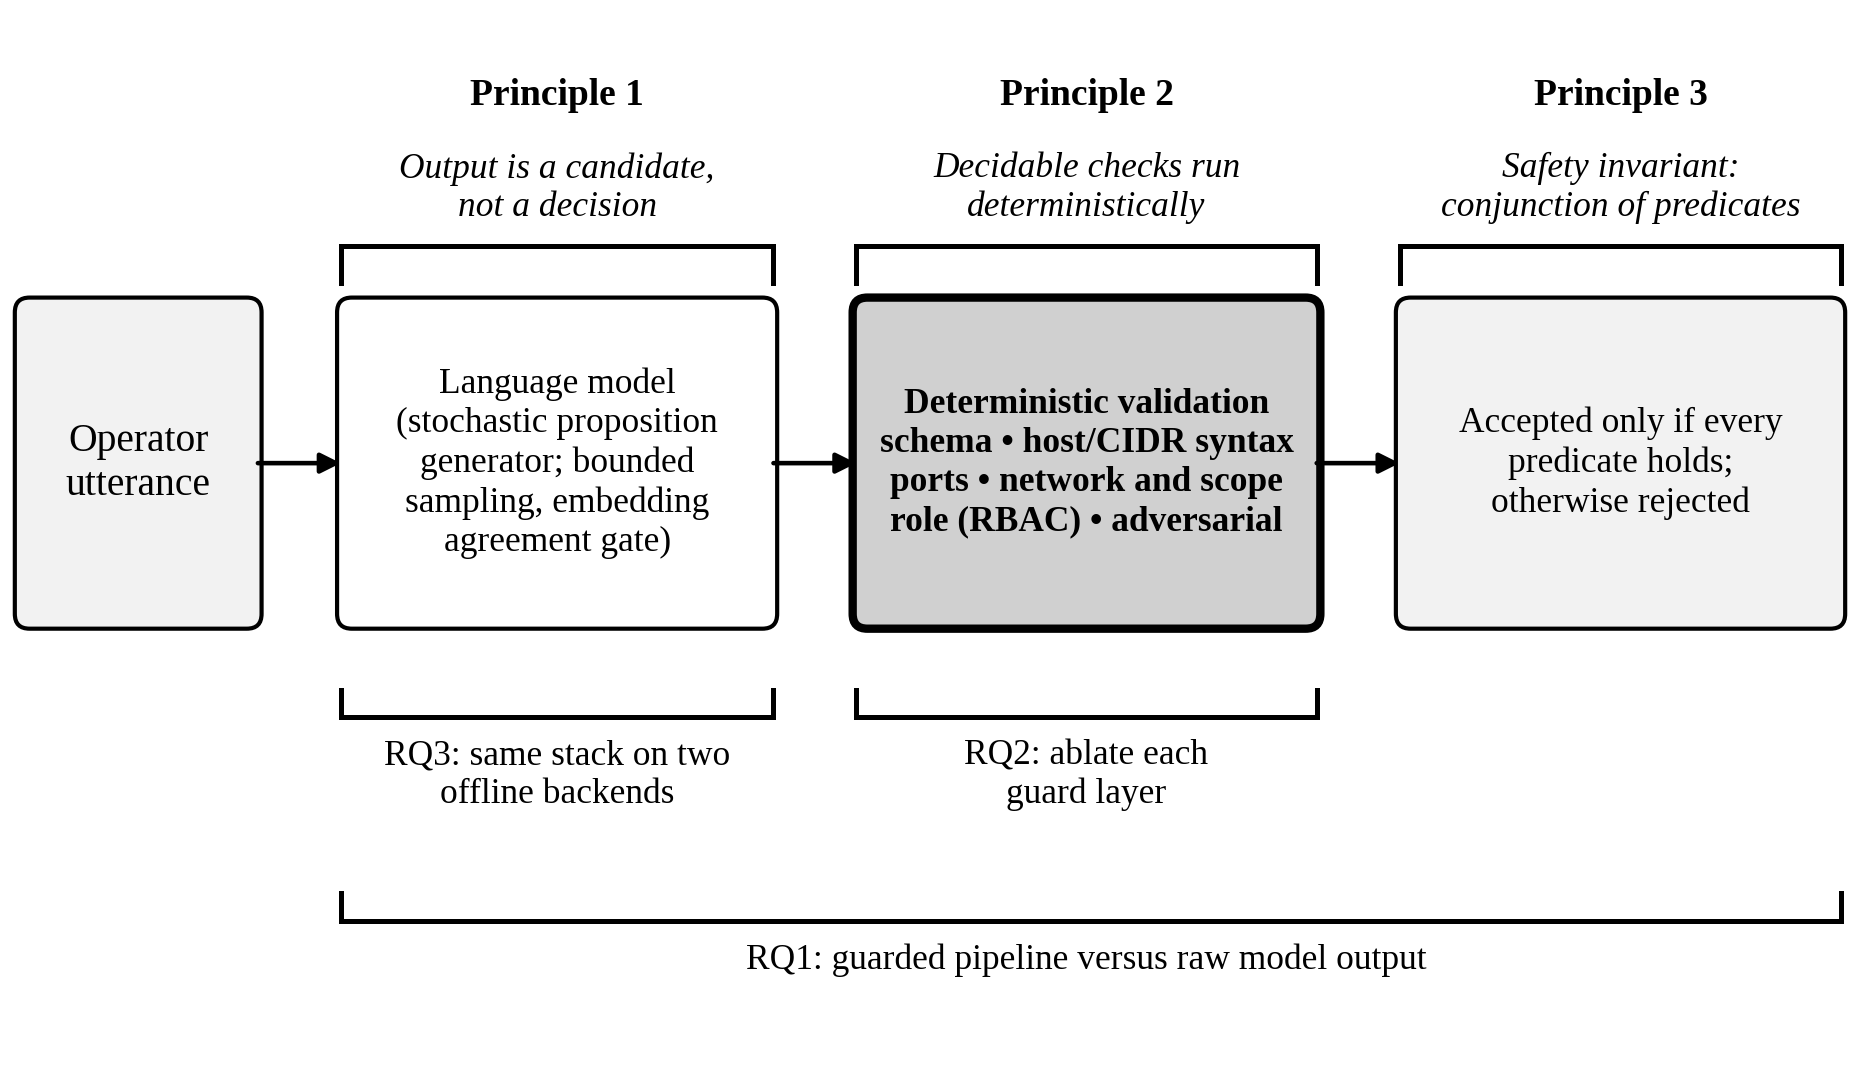
\includegraphics[width=0.9\textwidth]{C-01-Intetrecodnition Engine.pdf/vertopal_433ccb30063e47f1ba4c32a79683aeea/media/image3.png}
  \caption{Conceptual framework of the IRE within the NeuroShell chain: from the
  request to the guarded intent contract that downstream components consume.}\label{fig:conceptual}
\end{figure}

These principles enter the design formally. The IRE defines a guarded decision
function \(\Phi\) over the input utterance \(x\), and the safety invariant that
an intent is accepted only when the conjunction of the deterministic predicates
holds:
\[
  \mathit{Accepted}\bigl(\Phi(x)\bigr)\;\Longrightarrow\;
  \bigwedge_{k \in K} P_{k}(x),
  \qquad K=\{S5,S6,S6B,S7,\mathrm{RBAC},M1\},
\]
where each \(P_k\) is a deterministic predicate (schema, regex, network,
scope, authorisation, and adversarial-input checks) that is recomputed without
further model calls. The same safety-by-predicate attitude appears in the
planner's validation and safety filters, the AEERE's three checks applied to
every fixed command, and the AVAE's feature-grounded scoring.

\section{Research Gap}\label{sec:gap}

\subsection{Gaps in Offensive-Security Automation}\label{sec:gap-overall}

The literature is consistent on several limitations. First, existing AI security
copilots execute a plan but do not fix their own failures; an error message
terminates the run and requires human intervention. Second, most systems accept
natural language directly and pass model output to tools without a deterministic
safety boundary, so malformed, out-of-scope or adversarial content can reach a
live tool. Third, tool documentation is either embedded in the prompt or
unavailable, and command generation is not grounded in an explicit,
maintainable reference. Fourth, when findings are produced, they are typically
raw tool output: vulnerability intelligence is not combined with machine-learning
classification to prioritise what should be reviewed first. Fifth, almost all of
the surveyed systems rely on cloud-hosted models, which conflicts with
organisations whose policies require that commands, errors, and targets never
leave the premises.

\subsection{Gap Specific to Each Component}\label{sec:gap-percomponent}

For the IRE, the gap is the absence of a small, offline model combined with
deterministic validation to gate a security copilot; existing research either
uses unguarded output or relies on remote model safety. For the planner, the gap
is the translation of an explicit structured intent into a validated command,
grounded in documentation and checked against explicit validation and safety
constraints. For the AEERE, the gap is the handling of tool failure: no surveyed
system reads a failed security tool's error, labels it, and writes a fixed
command by itself, and none does so fully on the machine. For the AVAE, the gap
is integrating scanner-output parsing, vulnerability intelligence, an
exploitation-evidence classifier, and explainable prioritisation into a single
analysis workflow that operates within an autonomous assessment chain.

\section{Research Problem}\label{sec:problem}

\subsection{Framework Problem Statement}\label{sec:problem-overall}

The overarching problem addressed by this research is how to move from a
natural-language security request to an explainable, prioritised vulnerability
report with minimal human intervention, while keeping every step within a
controlled safety boundary. Concretely: how can a framework translate a request
into a validated intent, plan a grounded command, execute and recover that
command autonomously in a sandbox, and finally analyse the results, such that no
insecure operation is ever emitted and no operational data leaves the local
environment?

\subsection{Problem Specific to Each Component}\label{sec:problem-percomponent}

Each component addresses a distinct sub-problem. The IRE must translate
free-form instructions into validated intent contracts while rejecting
malformed, hallucinated, out-of-scope, and adversarial utterances. The planner
must translate a structured cybersecurity intent into a command that accurately
represents the requested operation and satisfies the constraints of the
supported tool environment, preserving target and parameters through
generation. The AEERE must read a failed security tool's error, understand it,
and write a fixed command by itself, with no human help, under a sandbox and
safety policy. The AVAE must process security assessment outputs and prioritise
vulnerabilities using exploitation evidence while keeping predictions
explainable.

\section{Research Objectives}\label{sec:objectives}

\subsection{Main Objective}\label{sec:objectives-main}

The main objective of this research is to design, develop, and evaluate
NeuroShell, an autonomous natural-language-driven orchestration framework for
offensive security operations, in which four cooperating components convert a
natural-language request into validated intents, grounded commands, sandboxed
execution with autonomous error recovery, and explainable vulnerability
prioritisation---with all model inference performed locally.

\subsection{Specific Objectives per Component}\label{sec:objectives-specific}

The following specific objectives were established across the four components:

\begin{enumerate}
  \item To design a guarded intent-recognition pipeline that combines an offline
  language model with deterministic validation, and to author an annotated
  evaluation data set covering well-formed and deliberately flawed prompt
  categories, along with an evaluation harness and a per-layer ablation
  protocol (IRE).
  \item To design a planning workflow that processes the structured intent
  contract, to develop a retrievable knowledge base containing documentation for
  Nmap, Nikto, and Gobuster, to implement tool selection and
  documentation-grounded command synthesis, and to implement validation and
  safety checks over generated commands, exposed through an API (planner).
  \item To design and implement a sandboxed execution engine with a five-stage
  error-recovery loop, a three-step fast-to-slow error-labelling cascade that
  ends in a local AI model, an eight-type Kali-specific error list with
  retry limits and tool-swap rules, and three safety checks applied to every
  fixed command (AEERE).
  \item To prepare a structured vulnerability-intelligence data set, to develop
  scanner-output parsers for Nmap, Nikto, and Gobuster, to train and evaluate an
  XGBoost classifier using five vulnerability features, and to implement
  SHAP-based explainability, contextual prioritisation, Neo4j graph storage, and
  a FastAPI interface (AVAE).
\end{enumerate}

\subsection{Research Questions}\label{sec:rqs}

The component reports define research questions aligned with these objectives:

\begin{enumerate}
  \item \textbf{IRE:} Does a guarded, offline-language-model pipeline produce
  schema-valid, authorised, and in-scope intent contracts more reliably than raw
  model output, and which pipeline stage contributes most to safety?
  \item \textbf{Planner:} How accurately does the planner translate structured
  intents into commands that select the appropriate tool, preserve the supplied
  parameters, and use valid syntax; what effect does retrieval have on command
  correctness and latency; and how effectively do the validation and safety
  mechanisms reject invalid requests?
  \item \textbf{AEERE:} Can a system read a failed security tool's error,
  label it, and produce a fixed command by itself, and can it do so fast enough
  and without ever letting a dangerous command through?
  \item \textbf{AVAE:} How effectively can vulnerability-intelligence features
  support classification of vulnerabilities according to known exploitation
  evidence using XGBoost, and how well can SHAP explanations support
  interpretation and prioritisation?
\end{enumerate}

\section{Scope, Limitations and Assumptions}\label{sec:scope}

The framework is scoped to a defined tool set and a defined trust boundary. The
planner and the parsers support Nmap, Nikto, and Gobuster; the IRE supports these
three tools plus Nuclei. The AEERE builds and tests on a data set of 8,000
labelled Kali command-failure cases covering ten error types, more than eighteen
tools, and three difficulty levels. The AVAE builds its classifier on a
curated data set of 155,852 vulnerability records derived from public
vulnerability sources, with the classification target defined from CISA KEV
membership. All model inference is performed locally through Ollama; no command,
error text, or target is transmitted off the deployment machine.

Several limitations bound the generality of the results. Natural-language intent
recognition is the responsibility of Component~1; the planner consumes the
resulting structured contract rather than performing the complete
interpretation of the original request. Findings for the planner are limited to
the supported tools, documented options, and cases included in the evaluation.
The AEERE's data set is hand-built, so real-world terminal errors may behave
differently. The AVAE model relies on five structured features and a
KEV-derived target, so its predictions reflect relationships within the
available data. Most evaluation data are single-run point estimates obtained on
limited hardware, and no component completed a formal user or stakeholder
validation study. The framework assumes that all test targets are private,
RFC-1918 lab addresses that cannot reach any real system.

\section{Thesis Structure}\label{sec:structure}

This combined dissertation is organised into four chapters. \cref{ch:methodology}
presents the research methodology and the design of the framework, including the
research approach, the architecture, the ethical and safety measures, the
commercialisation aspects, and the testing and implementation strategy.
\cref{ch:results} reports the results and findings of each component, together
with a discussion and a summary of each student's contribution.
\cref{ch:conclusions} concludes the study, assesses the achievement of the
objectives, and identifies recommendations and future work. The appendices
provide the research instruments used by each component and the disclosure of
AI usage.
\chapter{Methodology}\label{ch:methodology}

\section{Methodology}\label{sec:methodology}

\subsection{Overall Research Approach}\label{sec:method-approach}

The four component studies adopt a Design Science Research (DSR) approach. This
method suits computer-science projects whose goal is to build something new and
demonstrate that it works: instead of studying a problem only in theory, the
researchers build a real, working system and test it. The DSR cycle used
throughout the project has four steps. First, understand the problem through the
literature review, which shows that no current system combines guarded intent
recognition, grounded planning, autonomous error recovery, and local
vulnerability analysis. Second, build the artefact: each component is
implemented as a working service with a defined interface contract. Third, test
the artefact on purpose-built data sets and measure the relevant quality
attributes. Fourth, report the design choices, the results, and the findings.

A controlled design-and-evaluation protocol was committed in advance. Each
component fixed its data-set construction, its evaluation measures, and its
comparison configurations before reporting results, and each component exposes
its committed artefacts (prediction files, test logs, and configuration) so that
the reported figures can be audited.

\subsection{Framework Architecture and Requirements}\label{sec:method-arch}

NeuroShell is organised as a four-component chain. \cref{fig:arch-ire} positions
the IRE within the stack; the identical chain is described in each component
report.

\begin{figure}[htbp]
  \centering
  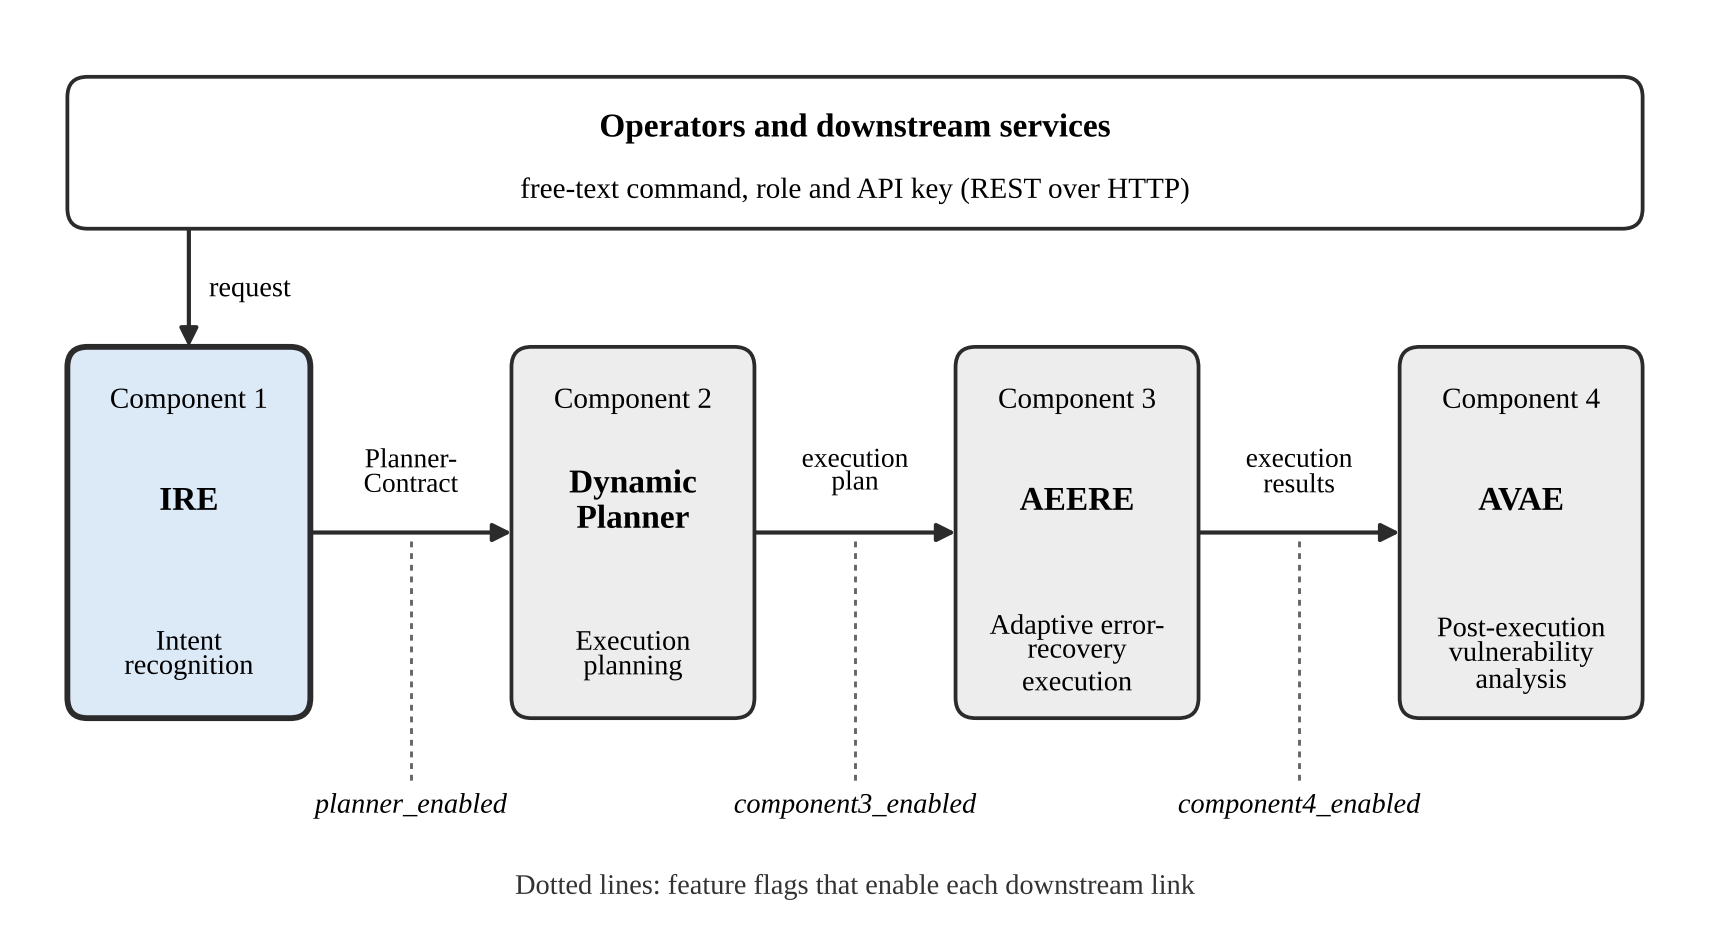
\includegraphics[width=0.9\textwidth]{C-01-Intetrecodnition Engine.pdf/vertopal_433ccb30063e47f1ba4c32a79683aeea/media/image6.png}
  \caption{Position of the Intent Recognition Engine within the NeuroShell
  four-component stack.}\label{fig:arch-ire}
\end{figure}

Each component is an independent FastAPI service that shares state through
Redis and communicates through structured JSON over HTTP. The IRE exposes the
entry point (port 8001) accepting natural language; the planner (port 8002)
accepts the intent contract and returns a validated command; the AEERE (port
8003) executes commands in a Docker sandbox and returns execution records; the
AVAE (port 8004) accepts execution records and returns structured, prioritised
vulnerability findings. \cref{tab:chain} summarises the four parts.

\begin{table}[htbp]
  \centering
  \begin{tabular}{@{}p{0.28\textwidth}p{0.68\textwidth}@{}}
    \toprule
    \textbf{Component} & \textbf{Job}\\
    \midrule
    C1 --- Intent Recognition Engine & Reads the plain-English request and
    turns it into structured JSON with the intent and details (port 8001).\\
    C2 --- Dynamic Planner \& RAG Engine & Turns the intent into a command by
    reading a store of tool documentation (port 8002).\\
    C3 --- Adaptive Execution \& Error-Recovery Engine & Runs the command in a
    sandbox, records the output and errors, and fixes failures on its own (port 8003).\\
    C4 --- AI-Driven Vulnerability Analysis Engine & Takes the logs from C3,
    finds weaknesses, and predicts how risky they are (port 8004).\\
    \bottomrule
  \end{tabular}
  \caption{The four parts of NeuroShell and their responsibilities.}\label{tab:chain}
\end{table}

\subsection{Methodology of the Intent Recognition Engine}\label{sec:method-ire}

The IRE methodology is a controlled design-and-evaluation study under a
committed protocol. The data set is a purpose-built, annotated collection of
1,500 security prompts: 600 well-formed records and 900 deliberately flawed
records spanning eight flaw classes (adversarial utterances, RBAC violations,
fabricated parameters, type mismatches, fabricated CVEs, contradictory
requests, out-of-scope targets, and ambiguous requests). Every record carries a
committed ground-truth label so that per-record decisions can be scored
deterministically.

The artefact is a seven-stage pipeline wrapped in five middleware components
(see \cref{fig:ire-pipeline}): the raw output of an offline language model is
parsed into a proposition, then validated for structure, target syntax, and
authorisation before an intent contract is emitted. Middleware adds the
authorisation checks, an adversarial-utterance detector, and a
hallucination-validation gate that enforces the safety invariant that every
accepted intent is schema-valid, authorised, and in scope.

\begin{figure}[htbp]
  \centering
  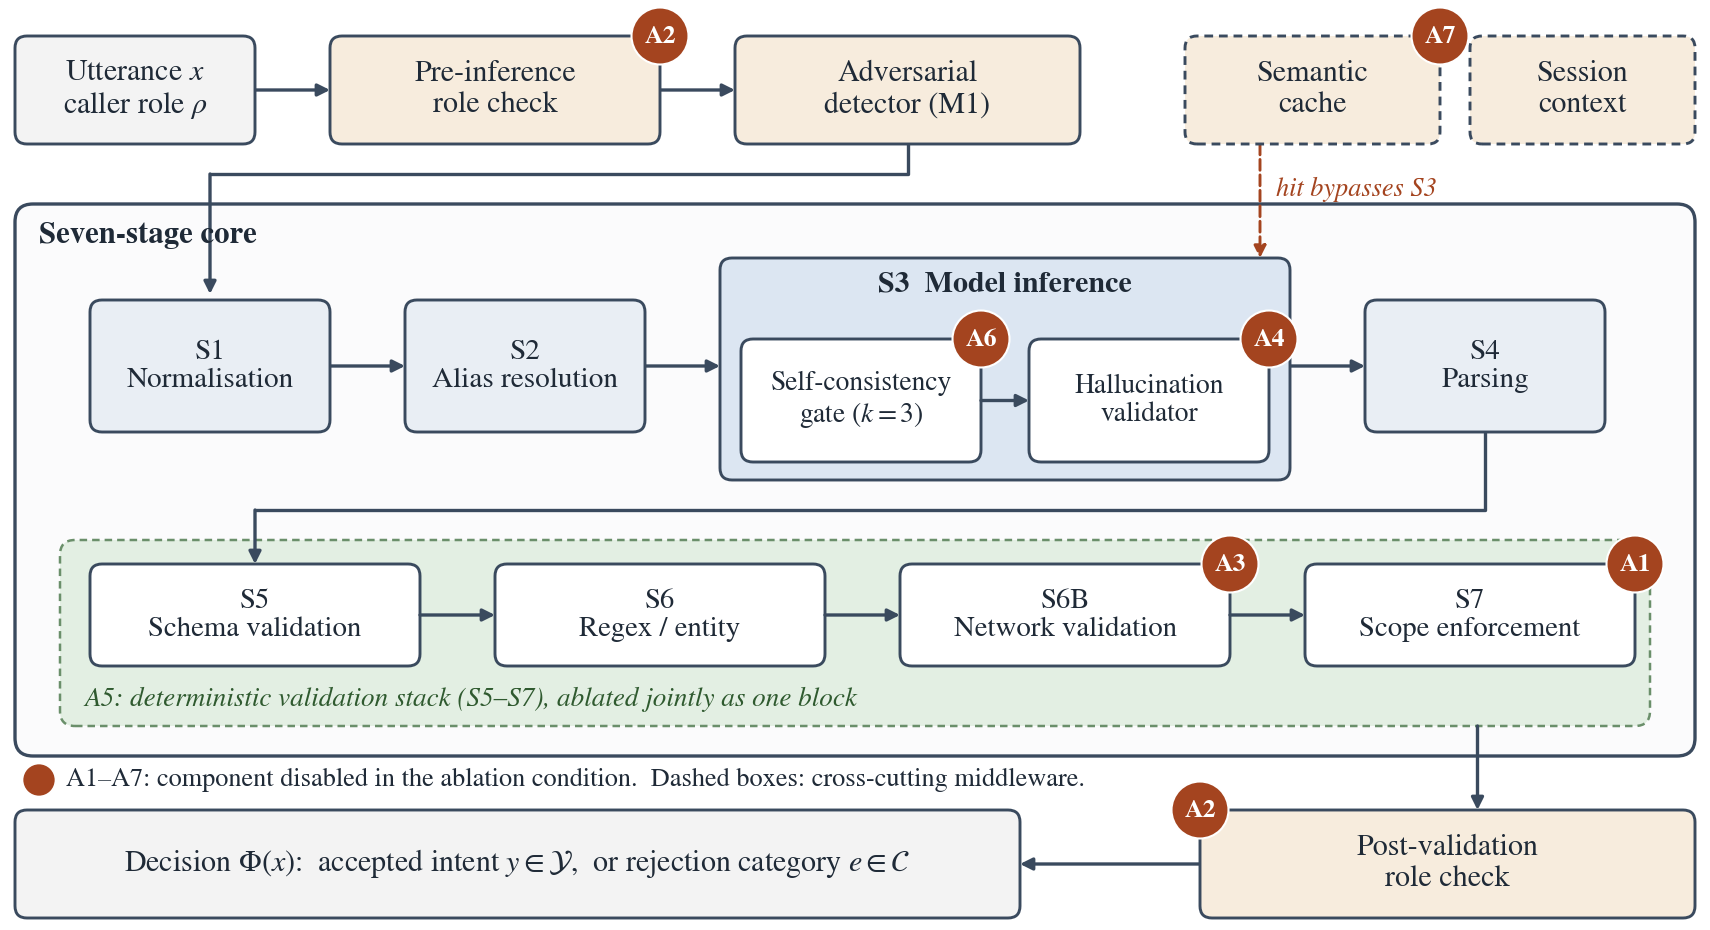
\includegraphics[width=0.9\textwidth]{C-01-Intetrecodnition Engine.pdf/vertopal_433ccb30063e47f1ba4c32a79683aeea/media/image4.png}
  \caption{The guarded pipeline of the IRE and the ablation protocol used to
  quantify the contribution of each layer.}\label{fig:ire-pipeline}
\end{figure}

Four experiments are defined. Experiment~1 measures the value of the whole
pipeline against raw model output. Experiment~2 compares two offline backends
(Gemma and Qwen) under an identical guardrail stack. Experiment~3 performs a
per-layer ablation in which one protection is removed at a time to quantify each
layer's contribution to safety. Experiment~4 reports the catch rate for each
flaw class separately. All results are single-run point estimates obtained on
one CPU-only machine, which limits cross-platform generalisation.

\subsection{IRE Architecture and Requirements}\label{sec:method-ire-req}

The IRE is a modular Python service with a FastAPI interface, running as a local
daemon under the Uvicorn ASGI server on port 8001. Its source tree comprises ten
packages under \emph{src/} (among them \emph{api}, \emph{integration},
\emph{middleware}, \emph{pipeline}, and \emph{validation}), with central
configuration in \emph{config/}. Role-based access control (RBAC), enforcement
and feature policies are held in separate Python modules and a YAML file, and
runtime constants are loaded from the environment and the YAML flags at start-up,
so that every experimental constant is reproducible from the committed
configuration. A health start-up gate checks the environment file, Ollama
connectivity (port 11434) and model availability before serving.

The requirements were specified against the IEEE 830 recommended practice for
software requirements specifications. \cref{tab:ire-fr} lists the functional
requirements of the IRE grouped under four product functions, each with the
component that realises it, and \cref{tab:ire-nfr} states the non-functional
requirements with the design provision that satisfies each one. The functional
requirements establish a direct trace from ``what the component must do'' to the
pipeline stage or middleware that implements it, which is the basis for the
verification gate described later.

\begin{table}[htbp]
  \centering
  \begin{tabular}{@{}p{0.14\textwidth}p{0.07\textwidth}p{0.45\textwidth}p{0.20\textwidth}@{}}
    \toprule
    \textbf{Group} & \textbf{ID} & \textbf{Requirement} & \textbf{Realised by}\\
    \midrule
    Core understanding & FR-1 & Normalise the input utterance. & S1 Input Normaliser\\
    & FR-2 & Resolve offensive-security aliases (for example \emph{EternalBlue} to CVE-2017-0144) to canonical identifiers. & S2 Alias Resolver\\
    & FR-3 & Classify the request into one of nine top-level intents. & S3 inference; S5 schema validation\\
    & FR-4 & Refine the intent into a hierarchical sub-intent that drives downstream tool selection. & Sub-intent classifier; Contract Builder\\
    Safety and security & FR-5 & Detect adversarial input before inference. & M1 Adversarial Detector\\
    & FR-6 & Enforce role-based access control both before and after inference. & M2 and M5 RBAC Guard\\
    & FR-7 & Validate model output against typed-schema, regular-expression, network and engagement-scope rules. & S5, S6, S6B and S7\\
    & FR-8 & Classify every failed validation into one of six hallucination classes. & Enforcement policy\\
    & FR-9 & Emit an audit record for every parse. & Audit logger\\
    Intelligence and quality & FR-10 & Maintain per-session context across turns. & M3 Session Context\\
    & FR-11 & Serve identical intents from a semantic cache. & M4 Semantic Cache\\
    & FR-12 & Gate low-confidence decisions through a self-consistency stage. & Self-consistency stage\\
    & FR-13 & Provide an optional XAI attribution path (disabled by default). & Feature flag only\\
    System and integration & FR-14 & Expose a REST API for parsing, execution and administration. & REST API\\
    & FR-15 & Push validated contracts to downstream components on a feature-flagged basis. & Contract Builder\\
    & FR-16 & Persist an append-only audit trail. & Audit logger\\
    & FR-17 & Make every guard individually disable-able through configuration. & Feature-flag configuration\\
    \bottomrule
  \end{tabular}
  \caption{Functional requirements of the IRE and the stages/middleware that
  realise them (from the IEEE 830-based requirements specification).}\label{tab:ire-fr}
\end{table}

\begin{table}[htbp]
  \centering
  \begin{tabular}{@{}p{0.15\textwidth}p{0.45\textwidth}p{0.29\textwidth}@{}}
    \toprule
    \textbf{Attribute} & \textbf{Requirement} & \textbf{Design provision}\\
    \midrule
    Performance & Adversarial detection completes in low milliseconds; RBAC fast-fail runs before any model cost; cache hits short-circuit the pipeline. & Lightweight lexical and structural scoring in M1; M2 placed ahead of S3; M4 bypasses inference on a hit.\\
    Reliability & Failure in non-critical middleware (session context, cache, adversarial detection) degrades gracefully and does not abort the request. & S7 independently re-scans the raw input for injection, so losing M1 does not remove all injection screening.\\
    Security & The service holds no credentials beyond an operator API key; rate limiting protects the model backend; no free-form model output is ever returned. & Local daemon with a single shared API key; only schema-validated contracts leave the engine (S4 to S7).\\
    Operability & Every stage and middleware is configurable through feature flags; the model family and engagement scope are reconfigurable at runtime; evaluation is reproducible from a single manifest. & Administrative views for feature flags, models and engagement scope; an evaluation manifest that pins the sampling configuration.\\
    \bottomrule
  \end{tabular}
  \caption{Non-functional requirements of the IRE and the design provisions.}\label{tab:ire-nfr}
\end{table}

\subsection{IRE Detailed Design: Stages, Middleware and Enforcement}\label{sec:method-ire-design}

The IRE pipeline is organised as seven core stages wrapped in five middleware
components. Stages S1--S4 prepare the input and the model output. S1 normalises
casing, whitespace and Unicode (NFKC form) and standardises jargon terms into
canonical phrases. S2 resolves aliases, such as \emph{nmap -sS} to a SCAN action
and exploit names to canonical CVE identifiers, using the alias map in
\emph{data/alias\_map.json}. S3 instructs the model to emit a fixed JSON schema
at the sampling configuration pinned in the evaluation manifest. S4 recovers the
JSON payload by stripping code fences, markdown artefacts and thinking tags.

The remaining stages are deterministic validators, shown in
\cref{tab:ire-validators}. Because S5--S7 recompute every check without further
model calls, a model output can be exposed only if it satisfies all of them; the
deterministic guard path is therefore bit-exact and auditable, which is a
reproducibility property that the evaluation protocol relies on.

\begin{table}[htbp]
  \centering
  \begin{tabular}{@{}p{0.26\textwidth}p{0.69\textwidth}@{}}
    \toprule
    \textbf{Stage} & \textbf{Checks performed}\\
    \midrule
    S5 Schema Validator & Exactly one of nine \emph{IntentType} values; a matched target type; ports in the range 1--65535; CVE syntax \emph{CVE-YYYY-NNNN}; confidence in {[}0,1{]}; \emph{AMBIGUOUS} requires confidence below 0.5; \emph{REJECTED} requires a rejection reason.\\
    S6 Regex Validator & Deterministic re-verification of every entity produced by the model (IPv4 and IPv6 addresses, CIDR blocks, CVE identifiers, ports and URLs) and the absence of shell metacharacters.\\
    S6B Network Validator & Targets fall inside the configured engagement CIDR (default 192.168.0.0/16); permitted scan prefix lengths range from /30 (widest) to /32 (narrowest); target type is consistent with target value.\\
    S7 Scope Guard & Rejects out-of-scope targets in strict mode, warns in research mode; applies RFC 1918 private-address membership; re-scans the raw input as an injection gate.\\
    \bottomrule
  \end{tabular}
  \caption{Deterministic checks performed by the validation stages S5 to S7
  including S6B.}\label{tab:ire-validators}
\end{table}

The middleware provides the safety and quality functions around the core.
\cref{tab:ire-middleware} summarises the responsibilities of each middleware
component. The adversarial detector (M1) is a three-layer scorer: a lexical
layer scores known injection phrases and control tokens (weights 0.8--1.0), a
structural layer scores encoded payloads, script-like constructs and
imperative-but-unclassifiable phrasing (weights 0.3--0.9), and a scoring layer
fuses the signals into a cumulative score. A score at or above 0.7 flags the
request for downstream treatment and a score at or above 0.95 blocks it
immediately, before inference. Two-phase RBAC (M2 pre-inference, M5
post-inference) prevents a single bypassed guard from manufacturing an
authorised action; unknown roles are coerced to \emph{viewer}, the
least-privileged class. Session context (M3) maintains per-session turn history
with a time-to-live and injects the recent memory window into the prompt so that
anaphoric follow-ups such as ``the same target'' resolve correctly. The semantic
cache (M4) combines an exact hash with embedding similarity (sentence-transformers
\emph{all-MiniLM-L6-v2}) and short-circuits the LLM on a hit, pruning latency and
improving determinism; cache entries are invalidated together with the offline
CVE-grounding index so that cached decisions do not outlive the data they depend
on.

\begin{table}[htbp]
  \centering
  \begin{tabular}{@{}p{0.26\textwidth}p{0.68\textwidth}@{}}
    \toprule
    \textbf{Middleware} & \textbf{Responsibility}\\
    \midrule
    M1 Adversarial Detector & Three-layer lexical/structural/scoring gate before inference; flags at \(\ge0.7\), auto-blocks at \(\ge0.95\).\\
    M2 + M5 RBAC Guard & Two-phase authorisation around the core; unknown roles coerced to \emph{viewer}.\\
    M3 Session Context & Per-session turn history with TTL; memory window injected into the prompt.\\
    M4 Semantic Cache & Exact-hash plus embedding similarity; LRU-style eviction; invalidated with the CVE index.\\
    \bottomrule
  \end{tabular}
  \caption{The middleware components of the IRE and their responsibilities.}\label{tab:ire-middleware}
\end{table}

Every failed validation is classified into one of six hallucination classes and
recorded as an audit-grade \emph{ValidationFinding}. The enforcement policy maps
each class to one of three outcomes, BLOCK, WARN or ESCALATE
(\cref{tab:ire-hallucination}). Fabricated parameters, contradictory
action--target pairings, target-type mismatches and malformed fabricated CVEs
hard-block; ungrounded confidence (a syntactically valid but unindexed CVE)
warns; and out-of-scope targets warn in research mode but block in strict
production mode. Escalations are routed through an administrative escalation
queue for explicit human approval. This taxonomy is what lets the evaluation
report per-flaw-class catch rates rather than a single opaque rejection count.

\begin{table}[htbp]
  \centering
  \begin{tabular}{@{}p{0.28\textwidth}p{0.44\textwidth}p{0.19\textwidth}@{}}
    \toprule
    \textbf{Hallucination class} & \textbf{Description} & \textbf{Outcome}\\
    \midrule
    Fabricated parameters & Parameter values invented by the model. & BLOCK\\
    Contradictory action--target pairing & An action incompatible with the stated target. & BLOCK\\
    Target-type mismatch & A target value inconsistent with its declared type. & BLOCK\\
    Malformed fabricated CVE & An invented identifier that fails CVE syntax. & BLOCK\\
    Ungrounded confidence & A syntactically valid CVE absent from the offline index. & WARN\\
    Out-of-scope target & A target outside the declared engagement scope. & WARN in research; BLOCK in strict\\
    \bottomrule
  \end{tabular}
  \caption{Hallucination classes and their enforcement outcomes.}\label{tab:ire-hallucination}
\end{table}

\subsection{IRE Design Decisions}\label{sec:method-ire-decisions}

Seven principal design decisions shaped the IRE; each is recorded as a choice
between a credible alternative and the adopted design
(\cref{tab:ire-decisions}). Three of these decisions recur at framework level.
First, the decoder is local and CPU-only because a cloud-hosted model would
contradict the closed trust boundary. Second, output is a fixed validated JSON
schema rather than free-form prose, converting a plausibility claim into a
verifiable one. Third, validation is deterministic rather than model self-checked,
avoiding drift and reusing the same fallible estimator that produced the output.
The IRE additionally chooses \emph{no retrieval at inference time}: retrieved
text is itself a prompt-injection vector, so offline CVE grounding is loaded at
start-up only, keeping the threat model closed.

\begin{table}[htbp]
  \centering
  \begin{tabular}{@{}p{0.15\textwidth}p{0.25\textwidth}p{0.24\textwidth}p{0.25\textwidth}@{}}
    \toprule
    \textbf{Decision area} & \textbf{Alternative considered} & \textbf{Adopted design} & \textbf{Principal rationale}\\
    \midrule
    Decoder & Cloud-hosted model & Local model through Ollama, CPU-only & No request leaves the device; no credentials held\\
    Output form & Free-form prose & Fixed JSON schema validated by S4--S7 & Converts a plausibility claim into a verifiable one\\
    Validation & Model self-checking & Deterministic rules (S5--S7, S6B) & Avoids drift; bit-exact and auditable\\
    Grounding & Retrieval-augmented generation & No retrieval at inference time & Removes the retrieved-text injection vector\\
    Access control & Single post-hoc RBAC check & Two-phase RBAC (M2 and M5) & A bypassed guard cannot yield an authorised action\\
    Confidence & Single-pass model confidence & Self-consistency gate for low-confidence decisions & Calibrated scores are unreliable for small offline models\\
    Latency & Inference on every request & Two-channel semantic cache (M4) & Short-circuits repeated intents; improves determinism\\
    \bottomrule
  \end{tabular}
  \caption{The seven principal design decisions of the IRE.}\label{tab:ire-decisions}
\end{table}

The planner methodology follows the same DSR pattern with an explicit
experimental protocol. The planning workflow is organised into distinct stages:
intent interpretation, documentation retrieval, tool selection, command
synthesis, and validation. This separation makes the responsibility of each
stage explicit and allows the component to be developed and tested through
structured inputs without requiring the complete framework to be active for
every test.

The data set for the held-out assessment consists of 337 cases covering the
three supported tools (113 Nmap, 116 Nikto, and 108 Gobuster), each with a
reference command. Direct assessment compares the base and adapted
configurations on these held-out cases and reports strict exact-match rates by
tool. A separate 25-case experiment examines the base model with and without
retrieval, measuring semantic command accuracy, normalised exact-match rate,
tool-selection accuracy, and planning latency, isolating the effect of
documentation grounding. \cref{fig:planner-arch} shows the internal architecture
of the component.

\begin{figure}[htbp]
  \centering
  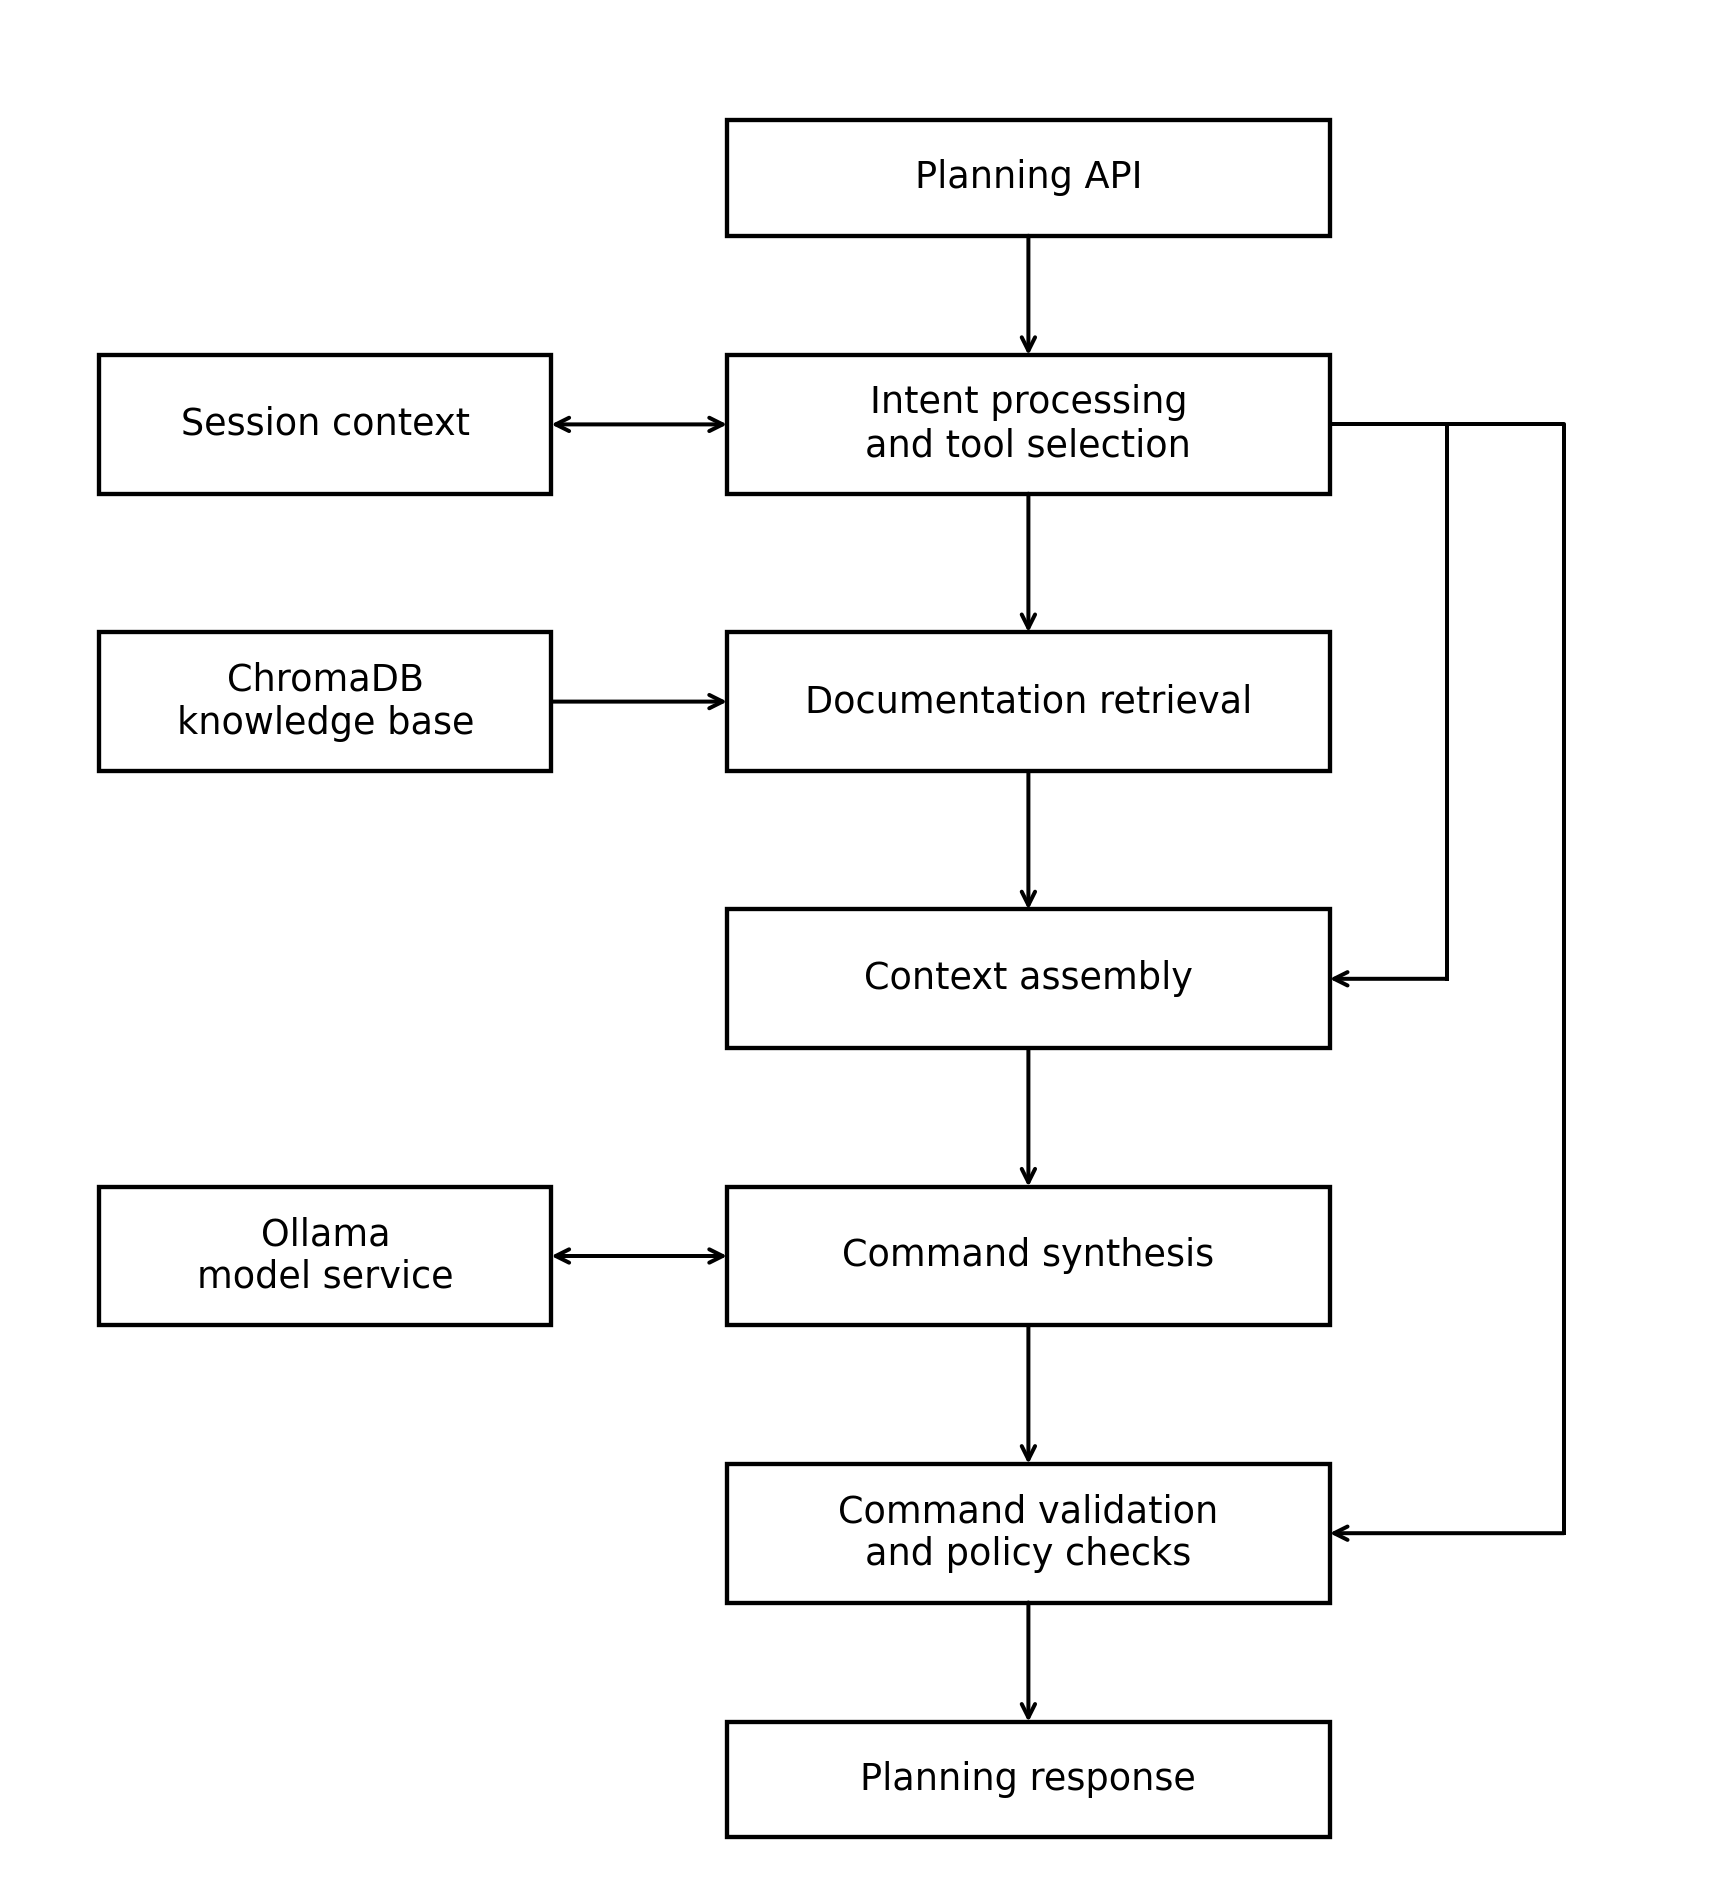
\includegraphics[width=0.85\textwidth]{C-02-Dynamic planner and rag enginee/vertopal_80eb40840323498cb949d017d9b2b63a/media/image2.png}
  \caption{Internal architecture of the Dynamic Planner and RAG Engine.}\label{fig:planner-arch}
\end{figure}

Measures and evaluation cover tool-selection accuracy, command syntax
correctness, semantic alignment, safety behaviour, and generation latency.
Rejection outcomes record whether the configured checks accept valid, in-scope
requests and reject invalid or out-of-policy requests. The knowledge base stores
documentation passages in ChromaDB with embeddings produced by
\emph{all-MiniLM-L6-v2}, and retrieval results are passed to the synthesising
model as context.

\subsection{Methodology of the Adaptive Execution and Error-Recovery Engine}\label{sec:method-aeere}

The AEERE was designed and tested using DSR. The engine works in five stages
that form a loop: run the command in a fresh Docker container running Kali
Linux; label the error; work out the cause; fix and check; and retry or stop
nicely. A fixed command returns to the run stage, and the cycle repeats until
the command works or the retry limit for that error type is reached. The engine
detects silent failures as well: a tool that exits with code 0 but produces no
useful output is treated as a failure (\cref{fig:aeere-loop}).

\begin{figure}[htbp]
  \centering
  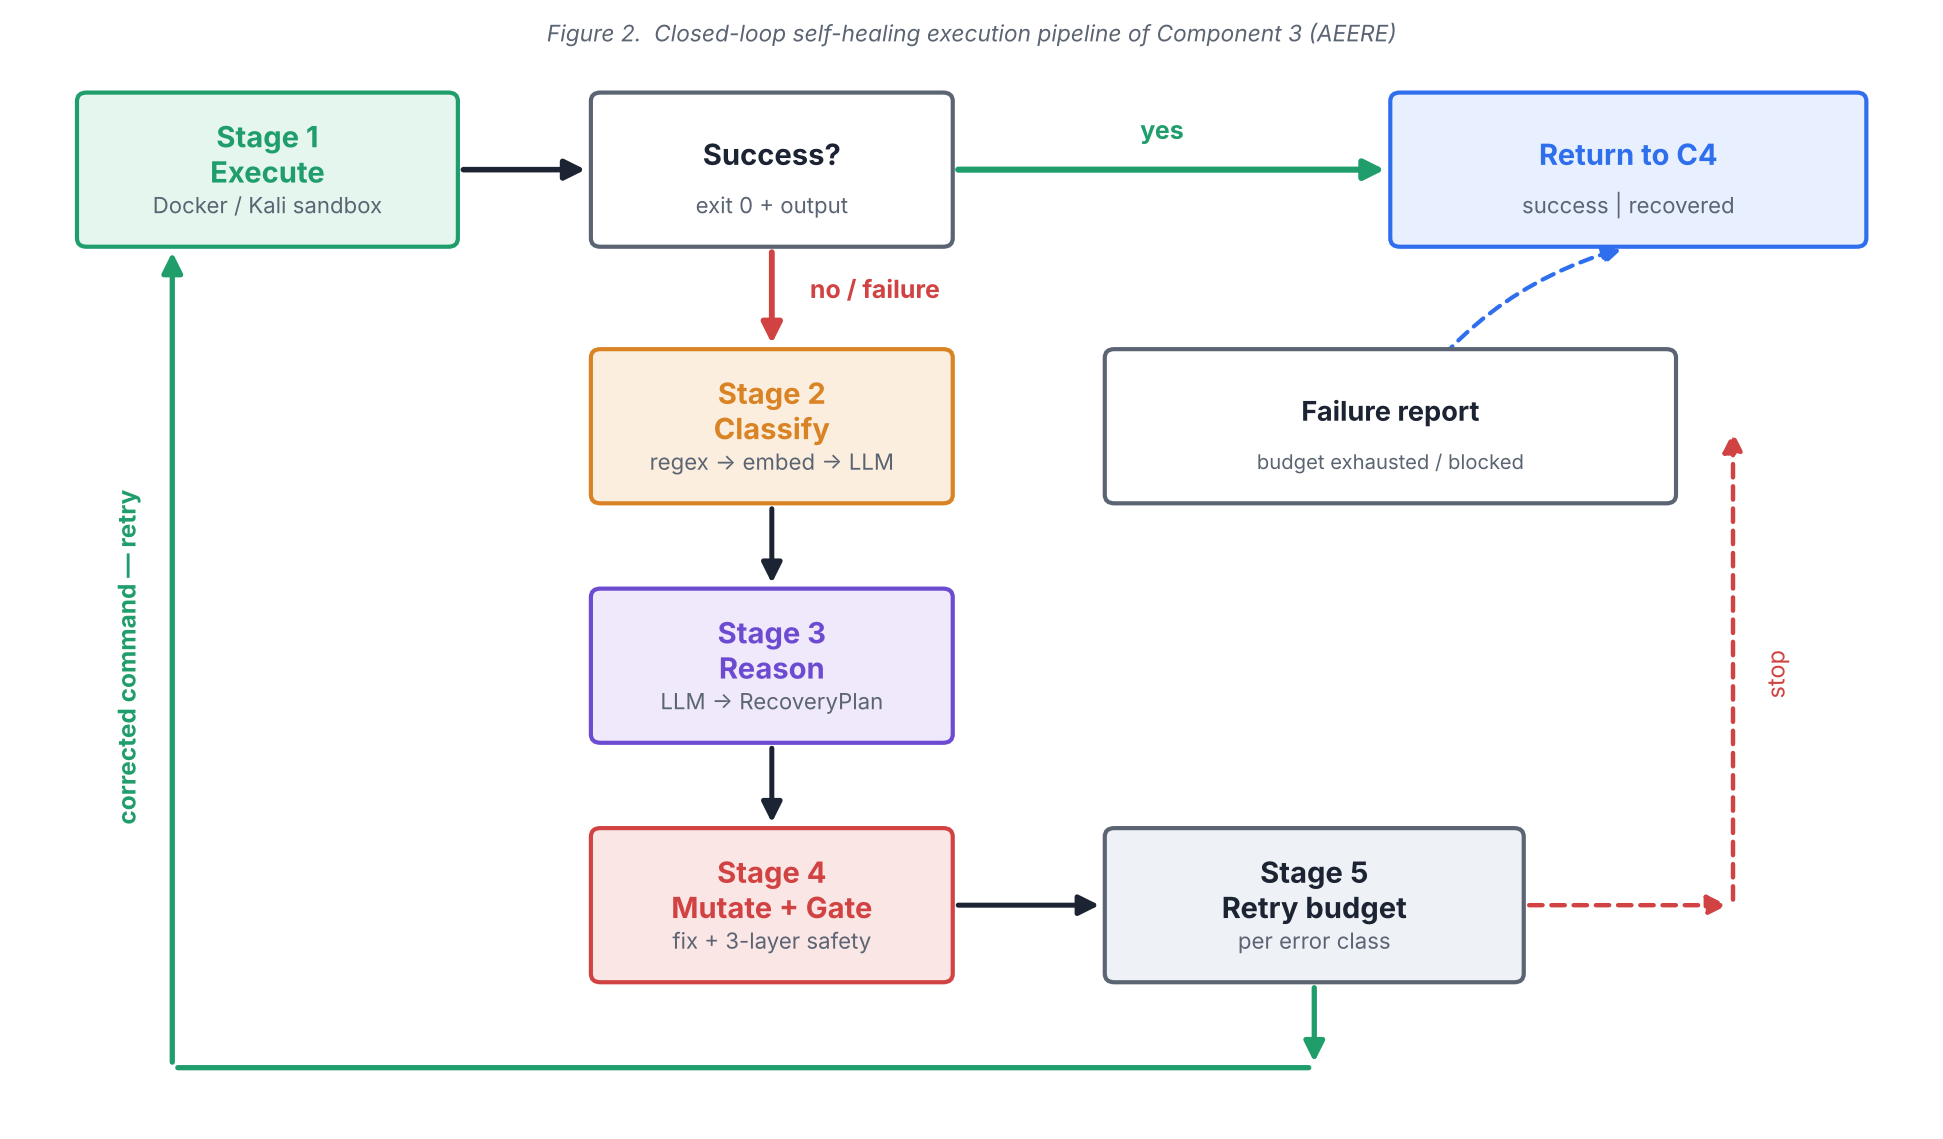
\includegraphics[width=0.9\textwidth]{C-03-Adoptive executer and error Recovery engine/vertopal_05e97fad080746c9b767567e93f99da6/media/image2.png}
  \caption{The five-stage error-recovery loop of the AEERE.}\label{fig:aeere-loop}
\end{figure}

Error labelling uses a three-step cascade that trades speed against thinking
power (\cref{fig:aeere-cascade}). Step 1 is a set of hand-written patterns tied
to an eight-type error list built specifically for Kali offensive-security tool
failures. Step 2 is a text-similarity check: a character n-gram TF-IDF vector
with logistic regression, trained only on the training half of the data set,
which accepts a match only above a 0.70 threshold. Step 3 is a local AI model
(Gemma run through Ollama) that receives the original command, the full error
message, the exit code, the possible error type, and task context, and replies
with a small JSON plan containing the cause, the chosen fix, and a corrected
command. The first step that labels the error stops the slower ones, so simple
errors stay cheap and fast.

\begin{figure}[htbp]
  \centering
  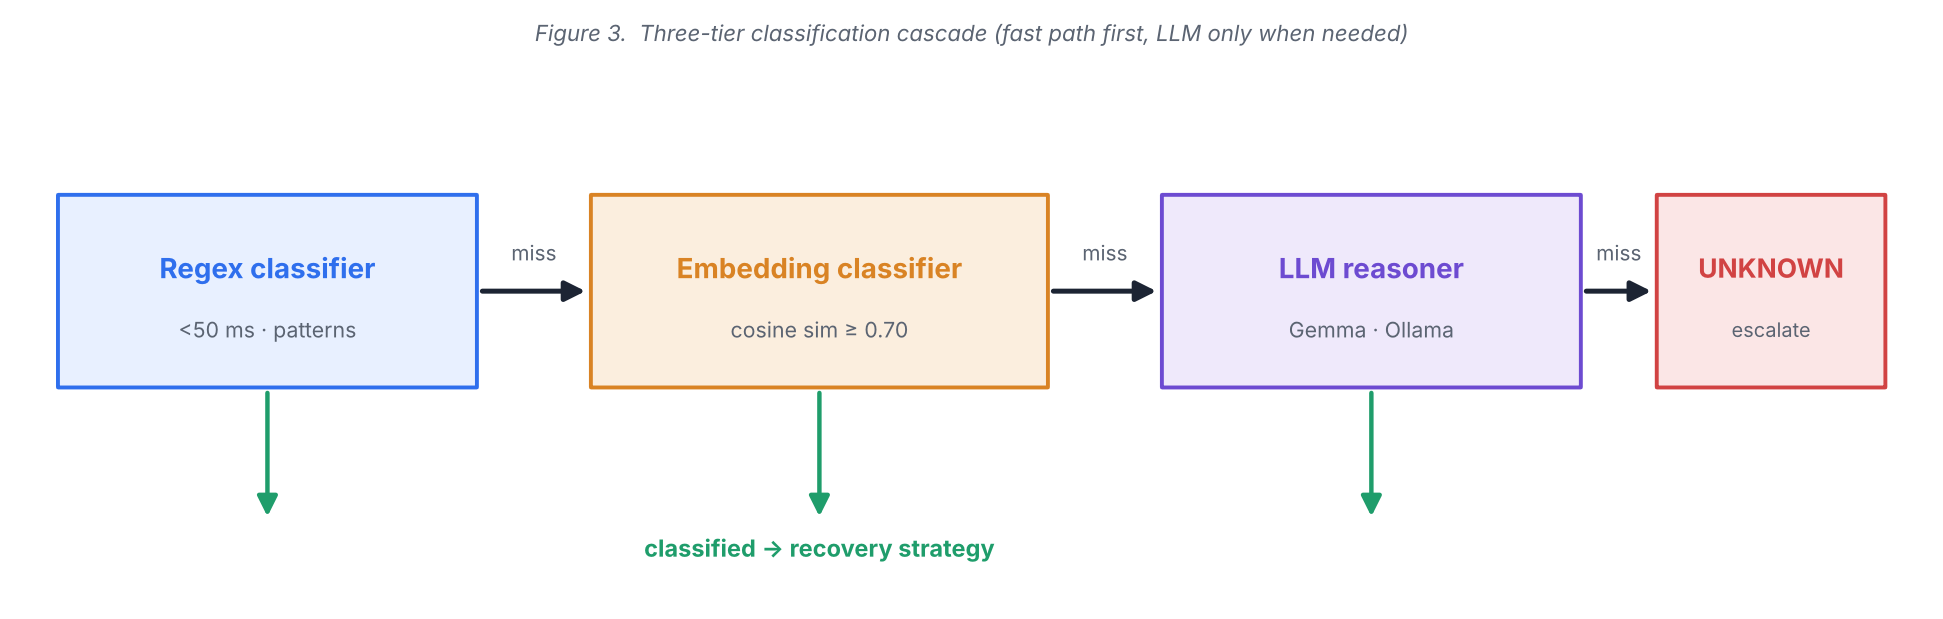
\includegraphics[width=0.9\textwidth]{C-03-Adoptive executer and error Recovery engine/vertopal_05e97fad080746c9b767567e93f99da6/media/image3.png}
  \caption{The three-step error check: fast path first; the AI is used only for
  new or unusual errors.}\label{fig:aeere-cascade}
\end{figure}

Every fixed command must pass three safety checks before it is allowed to run:
a format check on the AI's reply, a dangerous-word check that blocks destructive
or fetch-and-execute patterns (for example \texttt{rm -rf}, disk wiping, or
downloading and running code), and a confidence-and-scope check that requires a
minimum confidence level and rejects any target outside private RFC-1918 address
ranges. Every blocked case is written to a log in an SQLite database, which is
the evidence base for the safety tests.

The error list itself, shown in \cref{tab:aeere-errorlist}, is a contribution of
the work: it is the first of its kind for Kali offensive-security tool failures.
Each error type carries the example signs that point to it, the default fix, the
retry limit, and the wait rule. The engine also keeps a tool-swap list: when a
tool fails for good (its retry limit is used up), the engine swaps in a
different tool that does the same job, for example gobuster may be swapped for
ffuf or dirb for folder scanning, and nmap for masscan or rustscan for network
scanning, so the task can still finish.

\begin{table}[htbp]
  \centering
  \begin{tabular}{@{}p{0.18\textwidth}p{0.27\textwidth}p{0.27\textwidth}p{0.16\textwidth}@{}}
    \toprule
    \textbf{Error type} & \textbf{Example sign} & \textbf{Fix} & \textbf{Retries / wait}\\
    \midrule
    Tool not installed & command not found; exit 127 & Install with apt-get, then retry & 2 / fixed\\
    Permission denied & Permission denied; EACCES & Add sudo & 2 / fixed\\
    Network unreachable & No route to host; refused & Change timing / settings & 3 / growing\\
    Wrong syntax & Invalid option; usage: & Rewrite the flags & 2 / fixed\\
    Out of resources & Cannot allocate memory; ENOMEM & Lower threads / load & 2 / fixed\\
    Login failure & Authentication failed; publickey & Try another login method & 2 / fixed\\
    Timeout & ETIMEDOUT; timed out & Raise timeout / reduce scope & 3 / growing\\
    Version mismatch & deprecated; unknown option & Rewrite for the installed version & 1 / fixed\\
    \bottomrule
  \end{tabular}
  \caption{The eight error types of the AEERE error list and how each is
  fixed.}\label{tab:aeere-errorlist}
\end{table}

Building the test data set was a contribution in itself. There was no
ready-made public data set of Kali tool failures with correct fixes labelled,
so one was built: after planning for a minimum of 80 cases (at least ten per
error type), it was grown to 8,000 labelled command-failure cases. Each case
records the command, the raw error message, the exit code, the correct error
type, the cause, and the best fix. The data set covers ten error types, more
than eighteen tools (including netcat, gobuster, sqlmap, hashcat, nikto, ssh,
nmap, docker, dirsearch, and john), and three difficulty levels (2,663
beginner, 2,632 intermediate, and 2,705 advanced cases). All addresses in the
cases are private RFC-1918 lab addresses. \cref{fig:aeere-dataset} shows the
distribution across error types.

\begin{figure}[htbp]
  \centering
  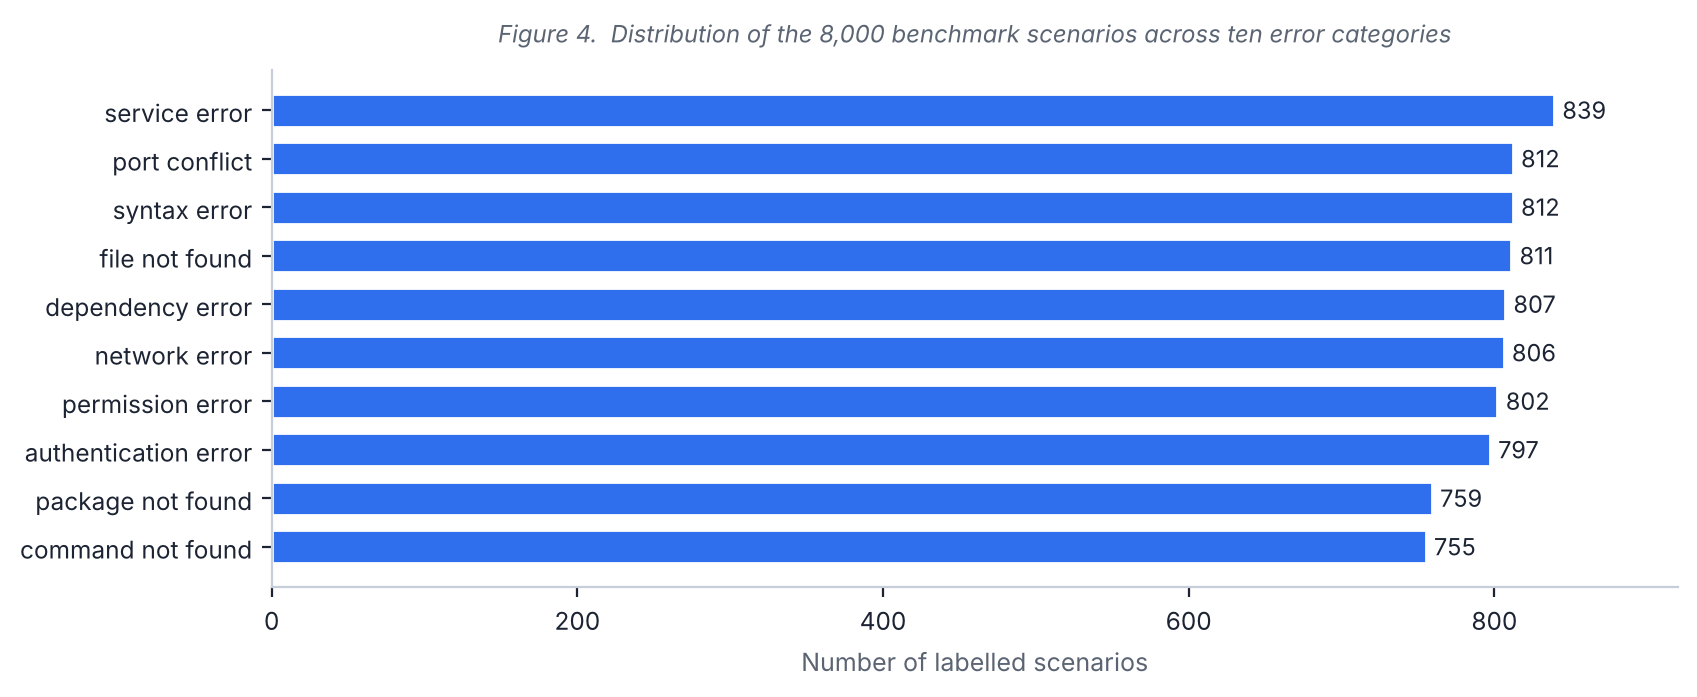
\includegraphics[width=0.9\textwidth]{C-03-Adoptive executer and error Recovery engine/vertopal_05e97fad080746c9b767567e93f99da6/media/image4.png}
  \caption{The 8,000 test cases spread across ten error types.}\label{fig:aeere-dataset}
\end{figure}

The error-labelling test was run in Python with scikit-learn. The 8,000 cases
were split into a training set (70\%, 5,600 cases) and a test set (30\%, 2,400
cases). The split was stratified so that every error type keeps the same share
in both halves, and a fixed random seed was used so the result can be repeated.
A second, harder test added controlled noise to each test message (log prefixes
and timestamps, trailing text, changed case, keyboard-style typos, and
truncation) with the noise level raised step by step from 0\% to 60\%, while the
text model remained trained only on the clean training half.

\subsection{Methodology of the AI-Driven Vulnerability Analysis Engine}\label{sec:method-avae}

The AVAE methodology combines vulnerability data preparation, feature
engineering, machine-learning model training, performance evaluation, and
component implementation. The primary data set is a curated collection of
155,852 vulnerability records derived from public vulnerability sources,
containing severity information, exploitation-related indicators, publication
details, and CISA KEV membership information. The NVD, CISA KEV catalogue, and
EPSS provide supporting intelligence. After cleaning (removing duplicates,
handling invalid values, converting attributes to numerical formats, and
computing vulnerability age from publication dates), the data set supported
154,889 class-0 records (no recorded KEV membership) and 963 class-1 records
(recorded KEV membership).

Feature selection produces five numerical features: CVSS v3 score, EPSS score,
EPSS percentile, vulnerability age, and an engineered interaction feature
computed as the product of the CVSS v3 score and the EPSS score. The
classification target is binary and derived from CISA KEV membership. XGBoost
was selected because it supports nonlinear relationships and efficient learning
from structured numerical data; hyperparameter tuning examined the number of
estimators, maximum tree depth, learning rate, minimum child weight, and
training-weight configuration, with validation performance (and specifically
PR-AUC) used to support model selection. SHAP was incorporated to describe the
contribution of individual features to the model's output, for both local
explanations of individual predictions and global feature-importance analysis.
Evaluation uses accuracy, precision, recall, F1-score, ROC-AUC, and PR-AUC,
together with a confusion matrix for error analysis.

The implemented component combines scanner-output parsing (Nmap, Nikto, and
Gobuster), vulnerability-intelligence enrichment, the trained classifier, SHAP
explanations, contextual risk prioritisation, Neo4j graph persistence, and a
FastAPI interface. \cref{fig:avae-shap} illustrates the feature-engineering
implementation used to prepare the model inputs.

\begin{figure}[htbp]
  \centering
  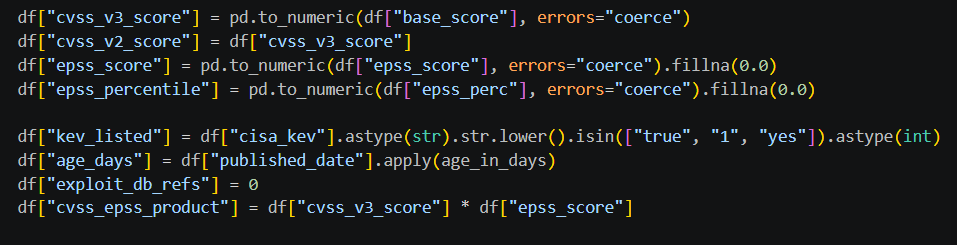
\includegraphics[width=0.9\textwidth]{C-04-AI-Driven Vulnerability Analysis Engine/vertopal_0d07bf200b61446895bb385b0aa02c6b/media/image3.png}
  \caption{Vulnerability-feature engineering implementation of the AVAE.}\label{fig:avae-shap}
\end{figure}

\subsection{Ethics, Privacy, Security, Standards and Responsible AI}\label{sec:method-ethics}

The safety properties of the framework were designed in, not added afterwards.
Four principles govern the deployment of NeuroShell:

\begin{description}
  \item[Sandboxed execution.] Every command runs inside a short-lived,
  locked-down Docker container; the real computer is never exposed. This
  protects against a fixed command harming the host.
  \item[Closed trust boundary.] All model inference runs on the local machine
  through Ollama. No command, error text, or target is transmitted off the
  device, which satisfies strict data-governance requirements of regulated and
  air-gapped environments and addresses the prompt-injection risk of connecting
  an agent to a live network~\cite{liu2023promptinjection}.
  \item[Authorisation and scope enforcement.] The IRE enforces role-based
  authorisation and engagement scope; the AEERE refuses commands that target
  public IP addresses, keeping all work inside RFC-1918 private ranges.
  \item[Test targets are private.] All assessment activity in the project was
  run against private lab addresses that cannot reach any real system, and
  crafted error output is cleaned before it enters an AI prompt to prevent
  prompt-tricking.
\end{description}

The project also follows established standards and frameworks. The development
and evaluation follow the design-science research tradition used across
computer-science theses. For AI governance, the work is aligned with the NIST AI
Risk Management Framework~\cite{nistairmf2023} and, where relevant, with secure
coding guidance such as the OWASP command-injection defence
cheat-sheet~\cite{owasp2025}. Responsible reporting is handled by disclosing the
use of AI assistance during writing and analysis (see
\cref{app:e}). No destructive operation is ever emitted, and every safety
rejection is logged for audit.

\emph{Standards and references shaping the design.} \cref{tab:standards}
records the standards and external references that shaped the design of the
framework, following the same traceability discipline used for the requirements.
The software requirements specification was written against the IEEE 830
recommended practice; the private-address enforcement of both the IRE (S7) and
the AEERE is grounded in RFC 1918; the threat catalogue that motivates the guard
stack follows the OWASP Top 10 for LLM Applications; offline CVE grounding draws
on the National Vulnerability Database as the canonical source of identifiers;
and the tool commands generated at the framework boundary follow the documented
syntax of the respective tools so that contracts are executable by the
downstream components.

\begin{table}[htbp]
  \centering
  \begin{tabular}{@{}p{0.36\textwidth}p{0.56\textwidth}@{}}
    \toprule
    \textbf{Standard or reference} & \textbf{Application in the design}\\
    \midrule
    IEEE 830 recommended practice for SRS & Structure of the requirements specification from which the requirements are derived.\\
    RFC 1918 & Private-address membership tests; restriction of targets to operator-declared private ranges.\\
    OWASP Top 10 for LLM Applications & Threat catalogue that motivates the guard stack.\\
    National Vulnerability Database & Canonical source of CVE identifiers for offline grounding.\\
    Nmap and Metasploit documentation & Syntax of the scanning and exploitation commands suggested in generated contracts.\\
    \bottomrule
  \end{tabular}
  \caption{Standards and references that shaped the NeuroShell design.}\label{tab:standards}
\end{table}

\section{Commercialization Aspects}\label{sec:commercial}

\subsection{Value Proposition and Target Users}\label{sec:commercial-value}

The value proposition of NeuroShell follows from its measured properties rather
than from asserted market figures. For security analysts and operators, the
framework removes manual intent-to-command translation, catches misremembered
syntax, out-of-scope targets, and role violations through deterministic
predicates rather than analyst vigilance, and produces structured responses and
per-request metrics that support audit. For security-tooling integrators, the
IRE exports a closed, schema-enforced contract (nine intent classes, validated
targets, explicit CVE, port, and modifier fields) that replaces prose
re-parsing in orchestrators. For offline-constrained environments, the
framework serves a segment that the surveyed cloud-based copilots do not: it
runs entirely on-device at inference, which is a differentiating fact for
air-gapped, regulated, edge, and research-range deployments.

\subsection{Market and Competitive Position}\label{sec:commercial-market}

The survey of existing systems found four categories (deterministic tooling,
generation-side copilots, tool-integration techniques, and post-hoc
guardrails), each strong in one respect and absent in another. NeuroShell, as a
whole, combines three properties none of the surveyed systems combine:
machine-consumed structured output, schema and scope enforcement, and offline,
CPU-only operation with autonomous error recovery. The AEERE targets the
specific gap left open by PentestGPT, VulnBot, and xOffense: no current AI
security tool fixes its own tool failures on the machine. The gap analysis is
review-based, because no named commercial product was surveyed; no market-share
or revenue claims are made.

\subsection{Business and Sustainability Model}\label{sec:commercial-business}

A business model is described as a set of candidate pathways rather than as
asserted revenue. Because all inference is local and CPU-only, operational
sustainability is low-cost and does not depend on per-call cloud fees. The
planner keeps its documentation store separate from the model, so the knowledge
base can be updated without retraining, which lowers maintenance cost. The
AEERE's error list and tool-swap list can be extended from logged UNKNOWN
errors, giving a data-driven path to keep the engine current as Kali tools
change. Licensing, pricing, and go-to-market details are outside the scope of
this dissertation and are left for a commercialisation plan.

\subsection{Scalability, Intellectual Property and Compliance}\label{sec:commercial-scalability}

The framework was designed to be modular: each component is independently
tested and deployed, which supports scaling out services horizontally. The IRE
and the AEERE run on CPU-only hardware and the AVAE model is small by design,
so the marginal infrastructure cost is low. Compliance-relevant properties
include the closed trust boundary (a strong data-protection argument), the
RFC-1918 scope restriction, and the SQLite audit logs of all safety rejections.
Intellectual-property considerations (patentability, licensing of the model
artefacts, and the documentation knowledge base) are flagged as open
requirements rather than asserted. Verified facts and open requirements are
separated in each component report, and no figure that was not measured is
claimed.

\subsection{Contribution to the Sustainable Development Goals}\label{sec:commercial-sdg}

NeuroShell contributes to several United Nations Sustainable Development Goals.
By automating security workflows and making them safe for less-experienced
operators, it supports building resilient infrastructure (SDG 9). By reducing
the labour and infrastructure cost of security assessment and by running on
shared, low-end hardware, it supports affordable and sustainable industrial
innovation. By protecting data on-premises through a closed trust boundary, it
supports strong institutions and the responsible use of technology. The
component reports map these contributions explicitly; as with all commercial
claims, the mapping is a narrative assessment rather than a measured outcome.

\section{Testing and Implementation}\label{sec:testing}

\subsection{Development Environment and Technology Stack}\label{sec:testing-stack}

All four components were developed in Python and deployed as FastAPI services.
Language-model inference uses Ollama with locally hosted models. The IRE
evaluates two backends (Gemma and Qwen); the planner adapts a Gemma~2 2B
instruction model (exported as a Q8\_0 GGUF artefact and imported into Ollama as
\emph{neuroshell-c2-gemma2-final}); the AEERE uses Gemma through Ollama; the
AVAE uses XGBoost and Scikit-learn. \cref{tab:stack} summarises the common
technology stack.

\begin{table}[htbp]
  \centering
  \begin{tabular}{@{}p{0.36\textwidth}p{0.60\textwidth}@{}}
    \toprule
    \textbf{Layer} & \textbf{Technology used across the framework}\\
    \midrule
    API layer & FastAPI (ports 8001--8004), shared state via Redis\\
    Language models & Gemma 2 2B (Q8\_0 GGUF) and Qwen via Ollama (local only)\\
    Tool documentation & ChromaDB vector store, \emph{all-MiniLM-L6-v2} embeddings\\
    Execution sandbox & Docker containers running Kali Linux\\
    Error-labelling & Hand-written patterns + char n-gram TF-IDF + logistic regression\\
    ML analysis & Pandas, Scikit-learn, XGBoost, SHAP, NumPy\\
    Persistence & SQLite (safety logs), Neo4j (vulnerability graph)\\
    Testing & pytest (unit and integration), pytest-asyncio\\
    \bottomrule
  \end{tabular}
  \caption{Consolidated technology stack of NeuroShell.}\label{tab:stack}
\end{table}

During development, the planner used a Colab environment for GPU-based
adaptation of the Gemma model and Ollama for local deployment; the framework is
intended to operate with local inference only. The model artefact is
approximately 2.8~GB on disk, which is a storage figure and not a minimum
runtime requirement.

\subsection{IRE Implementation, Verification and Testing}\label{sec:testing-ire}

The IRE was implemented as a module-based Python package under fastAPI. The
committed test suite comprises 506 tests (434 unit tests and 72 integration
tests), all of which pass against the current source, with statement coverage of
76\% overall. Coverage is further reported per module against the overall
figure. The evaluation protocol (four experiments, ablation; see
\cref{sec:method-ire}) is executed by a harness that commits per-record
decisions so figures can be audited. Two verified engineering findings were
recorded: a default development API key and an inactive \texttt{production}
scope mode, both flagged as gaps to close before deployment.

\subsection{Planner Implementation, Verification and Testing}\label{sec:testing-planner}

The planner backend was verified with a selected run of the committed test suite
on Windows with Python 3.11.9 and pytest 8.2.0: 42 tests passed with one warning
in 71.28 seconds. The warning concerns a pending deprecation in the \emph{multipart}
import used through Starlette and is not a test failure. The passing cases
support the implemented checks for malformed commands, target and port
contradictions, authentication behaviour, and session recovery. The test areas
and counts are shown in \cref{tab:planner-tests}.

\begin{table}[htbp]
  \centering
  \begin{tabular}{@{}p{0.50\textwidth}p{0.20\textwidth}@{}}
    \toprule
    \textbf{Test area} & \textbf{Passed tests}\\
    \midrule
    Planning API integration & 14\\
    Command validator & 3\\
    Safety filter & 4\\
    Intent interpreter & 6\\
    Command evaluator & 15\\
    \midrule
    Total & 42\\
    \bottomrule
  \end{tabular}
  \caption{Selected software verification results of the planner.}\label{tab:planner-tests}
\end{table}

\subsection{AEERE Implementation, Verification and Testing}\label{sec:testing-aeere}

The error-labelling test (SO3) was measured and is reported in
\cref{ch:results}: the three-step cascade reaches a macro-F1 of 100\% on the
clean data set and 99.1\% at 30\% message noise, remaining above 96\% even at
60\% noise. The pattern step runs in about 0.004~ms per message and the text
model in about 0.5~ms. The remaining verification targets (the overall fix rate,
the end-to-end speed and cost of a full fix, and the dangerous-command block
rate) require the full engine running on real hardware with Docker and Ollama,
which was not available at the time the component report was written. Those
tables are therefore recorded for the live engine; no result is invented. The
reported measurements are the labelling performance and per-step latency only.

\subsection{AVAE Implementation, Verification and Testing}\label{sec:testing-avae}

\begin{sloppypar}
Verification of the AVAE focuses on input processing, scanner-output parsing,
vulnerability-intelligence enrichment, machine-learning prediction, SHAP
explanation generation, API response handling, and graph persistence. Machine
learning verification evaluates the XGBoost classifier with the standard
classification metrics; software testing verifies that supported inputs are
processed correctly, relevant findings are extracted, and structured responses
are generated. The provisional model results are reported in \cref{ch:results}
with the explicit caveat, stated in the component report, that the final
conclusions require the confirmed, verified evaluation results.
\end{sloppypar}

\subsection{Integration Testing}\label{sec:testing-integration}

Integration testing verifies the hand-over between components. Selected API
tests passed for the planner's input handling, authentication, rejection, and
session-dependent target recovery. Local inference demonstrated an explicit Nmap
port request that produced \texttt{nmap -p 22,80,443 192.168.1.10} in both the
Colab adapter check and the Ollama check, and a service-detection request
produced \texttt{nmap -sV 192.168.50.10} locally. These are individual
generation checks rather than aggregate integration-accuracy measures. The AVAE
integration workflow verifies C3--C4 communication (structured execution-result
transfer), output parsing, ML prediction, SHAP explainability, Neo4j
integration, and API response generation. The complete integration outcome
across all four components requires confirmation through recorded end-to-end
testing evidence, which no single component report collects on its own.

\subsection{Deployment and Operation}\label{sec:testing-deploy}

Each component deploys as an independent FastAPI service. The IRE and the AEERE
use Ollama for local model inference (no cloud dependency). The planner imports
its adapted model as \emph{neuroshell-c2-gemma2-final} in Ollama and retains
ChromaDB as a persistent knowledge base. The AEERE requires Docker and Redis;
its \texttt{/execute} endpoint accepts a \texttt{PlannerOutput} and returns an
\texttt{ExecutionResult} with a status of \texttt{success}, \texttt{recovered},
or \texttt{failed}, a fix log, and a failure report, with a \texttt{/health}
check reporting whether the service and Docker are up. The AVAE loads its ML
artefacts at startup and exposes \texttt{/analyze} to receive structured
execution results and return analysis outputs. Because inference is local and
CPU-based, the framework can be operated on a single machine, which also
simplifies the operational sustainability model described in
\cref{sec:commercial-business}.
\chapter{Results and Discussion}\label{ch:results}

This chapter reports the results and findings earned by each component and
discusses what they mean, individually and as a chain. Each section first
states the measured results, then discusses them, then draws the conclusions
that feed the combined discussion in \cref{sec:results-discussion}.

\section{Results and Discussion of the Intent Recognition Engine}\label{sec:results-ire}

\subsection{Data set composition}\label{sec:results-ire-dataset}

\cref{tab:ire-flaws} shows the composition of the 1,500-record evaluation data
set. The well-formed subset (\(D^{+}\)) holds 600 legitimate requests across the
nine top-level intents, and the flawed subset (\(D^{-}\)) holds 900 records split
near-evenly across the eight flaw classes, so that per-class catch rates are
computed against classes of comparable size. This balance matters: because catch
requires an exact category match, borderline phrasings within a class are judged
against that class's own denominator rather than against a pooled rejection
count.

\begin{table}[htbp]
  \centering
  \begin{tabular}{@{}p{0.09\textwidth}p{0.31\textwidth}p{0.36\textwidth}p{0.13\textwidth}@{}}
    \toprule
    \textbf{Subset} & \textbf{Category} & \textbf{Description} & \textbf{Records}\\
    \midrule
    \(D^{+}\) & Well-formed requests & Legitimate requests, nine intents & 600\\
    \(D^{-}\) & Adversarial injection & Phraseology meant to divert the model & 113\\
     & Out-of-scope target/technique & Outside the declared engagement scope & 113\\
     & Ambiguous / under-specified & Too vague to resolve to one intent & 113\\
     & Contradictory request & Internally inconsistent requirements & 113\\
     & Fabricated parameter & Invented parameter values & 112\\
     & Fabricated CVE & Non-existent CVE identifiers & 112\\
     & Type mismatch & Phrasing mismatches the stated intent & 112\\
     & RBAC violation & Issued by an unauthorised role & 112\\
    \midrule
    & \multicolumn{2}{r}{Total \(D\)} & 1,500\\
    \bottomrule
  \end{tabular}
  \caption{Composition of the IRE evaluation data set.}\label{tab:ire-flaws}
\end{table}

\subsection{Experiment 1 (RQ1): value of the guarded pipeline}\label{sec:results-ire-exp1}

Experiment~1 compares raw model output against the full guarded pipeline on the
1,500-record data set. The results are consistent across both backends and are
summarised in \cref{tab:ire-exp1}.

\begin{table}[htbp]
  \centering
  \begin{tabular}{@{}lccc@{}}
    \toprule
    & \textbf{Decision accuracy} & \textbf{Catch rate} & \textbf{False-positive rate}\\
    \midrule
    Gemma, raw & 78\% & 0\% & 32\%\\
    Gemma, guarded & 86\% & 72\% & 14\%\\
    Qwen, raw & 69\% & 0\% & 31\%\\
    Qwen, guarded & 82\% & 64\% & 15\%\\
    \bottomrule
  \end{tabular}
  \caption{Experiment 1: raw versus guarded pipeline (full data set,
  \(N=1500\)).}\label{tab:ire-exp1}
\end{table}

The guarded pipeline raises decision accuracy from 78\% to 86\% for Gemma and
from 69\% to 82\% for Qwen (gains of 8 and 13 points), raises the flawed-input
catch rate from 0\% to 72\% and 64\% respectively, and lowers the
false-positive rate from 32\% to 14\% for Gemma and from 31\% to 15\% for Qwen.
The 0\% catch rate of raw output is expected: raw model output performs no flaw
classification, so a deliberately flawed prompt is accepted exactly like a
well-formed one.

\subsection{Experiments 2 and 3 (RQ2): backend comparison and ablation}\label{sec:results-ire-exp23}

The two backends behave similarly under the same guardrail stack and are close
apart in every measure that the framework can itself control. Gemma outperforms
Qwen in decision accuracy (86\% against 82\%) and in catch rate (72\% against
64\%); the false-positive rates are comparable (14\% against 15\%, a difference
within the noise band). Guarding also narrows the accuracy gap between the two
models from 9 points (78\% against 69\%) to 4 points, so the guardrail layer is
a leveller as well as a safety mechanism.

\cref{fig:ire-accuracy} shows Experiment~1 and the ablation results. The
per-layer ablation (Experiment~3) quantifies the contribution of each protection
to safety. \cref{tab:ire-ablation} reports the full ablation on both backends.
Removing the full validation stack has the largest single effect on catch rate:
30 points for Gemma (72\% to 42\%) and 24 points for Qwen (64\% to 40\%), with
virtually no change in the false-positive rate. Removing the adversarial-utterance
guard contributes most to the catch rate among the individual guards (9 points
for Gemma and 14 for Qwen), which is consistent with its role as the gate that
rejects the deliberately misleading sentences in the flawed set. Removing the
RBAC guard lowers both accuracy and catch rate in both models (by 7 points in
catch). Removing the hallucination gate or the semantic cache raises the catch
rate by 2--10 points but raises the false-positive rate sharply (to 30--44\%)
and lowers decision accuracy by 14--24 points, which shows that these layers
guard the well-formed side of the trade: they prevent valid requests from being
misclassified as flaws.

\begin{table}[htbp]
  \centering
  \begin{tabular}{@{}p{0.30\textwidth}rrrrrrr@{}}
    \toprule
    & \multicolumn{3}{c}{\textbf{Gemma}} & \multicolumn{3}{c}{\textbf{Qwen}}\\
    \cmidrule(lr){2-4}\cmidrule(lr){5-7}
    & \textbf{DAcc} & \textbf{Catch} & \textbf{FP} & \textbf{DAcc} & \textbf{Catch} & \textbf{FP}\\
    \midrule
    Full pipeline (baseline) & 86.0 & 72 & 14 & 82.0 & 64 & 15\\
    No scope guard & 65.0 & 74 & 42 & 68.0 & 68 & 30\\
    No RBAC guard & 75.0 & 65 & 20 & 57.0 & 57 & 17\\
    No network validator & 68.0 & 80 & 40 & 58.0 & 72 & 32\\
    No hallucination validator & 66.0 & 63 & 40 & 52.6 & 50 & 34\\
    No validation stack (S5--S7) & 65.0 & 42 & 15 & 62.0 & 40 & 16\\
    No self-consistency gate & 68.0 & 78 & 42 & 58.0 & 74 & 36\\
    No semantic cache & 67.0 & 77 & 44 & 60.0 & 70 & 40\\
    \bottomrule
  \end{tabular}
  \caption{Per-layer ablation (Experiment 3): each row removes one protection
  from the full pipeline. DAcc = decision accuracy; Catch = catch rate; FP =
  false-positive rate. Run-to-run noise is approximately \(\pm1\)--2 points.}\label{tab:ire-ablation}
\end{table}

\begin{figure}[htbp]
  \centering
  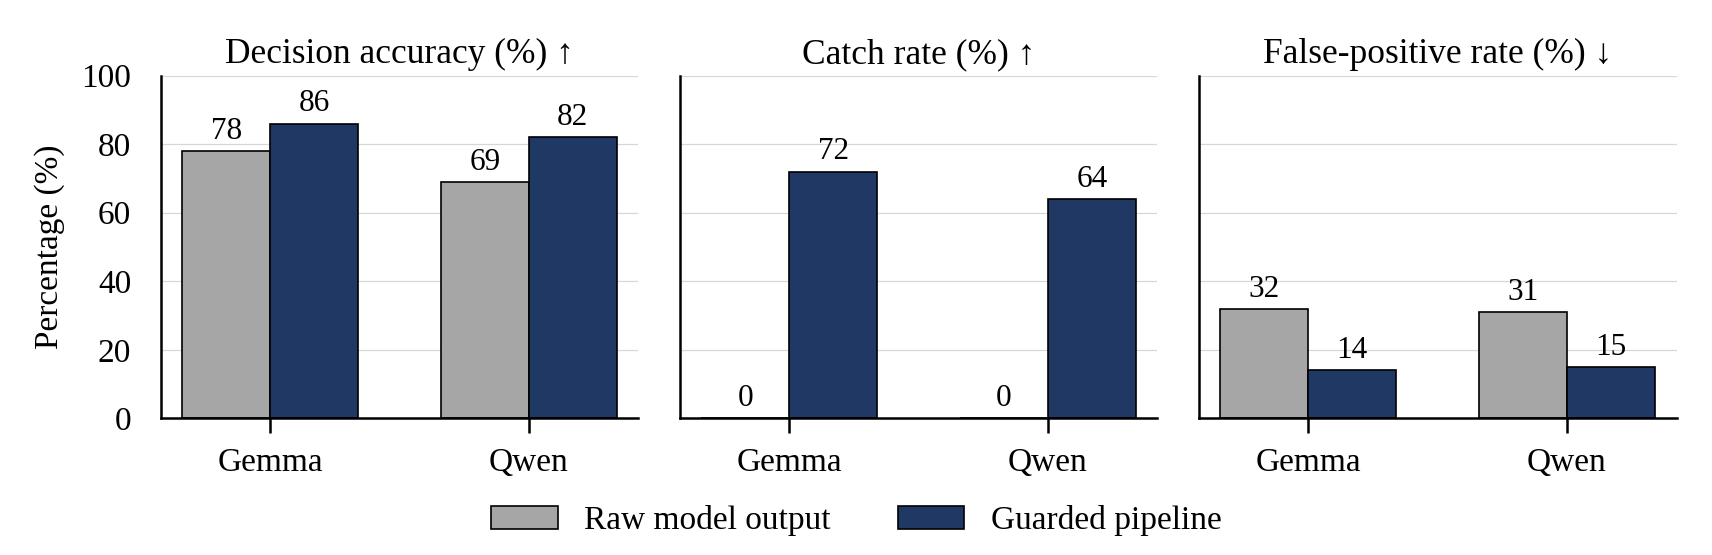
\includegraphics[width=0.9\textwidth]{C-01-Intetrecodnition Engine.pdf/vertopal_433ccb30063e47f1ba4c32a79683aeea/media/image10.png}
  \caption{Decision accuracy, catch rate and false-positive rate for raw and
  guarded configurations of both backends.}\label{fig:ire-accuracy}
\end{figure}

\subsection{Experiment 4 (RQ2): catch rate by flaw class}\label{sec:results-ire-exp4}

Experiment~4 reports the catch rate for each of the eight flaw classes
separately on a deep-dive subset, with each class evaluated on its own
denominator (\cref{tab:ire-perclass}). Catch is strongest where a deterministic
rule exists: RBAC violations are detected in 100\% of cases by the pre-inference
role check (M2), adversarial injections in 95.6\% by the adversarial detector
(M1), fabricated parameters (87.5\%) and type mismatches (81.3\%) by the
syntactic rules of S5--S6, and fabricated CVEs (78.1\%) by the offline grounding
of the hallucination validator. The residual weak classes are semantic:
contradictory (59.4\%), out-of-scope (46.7\%) and ambiguous requests (40.0\%)
offer no deterministic signal, so detection relies on the self-consistency gate.
These three classes account for 339 of the 900 flawed records (37.7\%) and
therefore weigh heavily on the overall catch rate. Because no confidence
intervals are available, class-level differences are indicative rather than
definitive.

\begin{table}[htbp]
  \centering
  \begin{tabular}{@{}p{0.36\textwidth}p{0.24\textwidth}p{0.34\textwidth}@{}}
    \toprule
    \textbf{Flaw class} & \textbf{Catch rate} & \textbf{Primary detection mechanism}\\
    \midrule
    RBAC violation & 100.0\% & M2 pre-inference role check\\
    Adversarial injection & 95.6\% & M1 lexical and structural detector\\
    Fabricated parameter & 87.5\% & S5--S6 syntactic rules\\
    Type mismatch & 81.3\% & S5--S6 syntactic rules\\
    Fabricated CVE & 78.1\% & Hallucination validator, offline grounding\\
    Contradictory request & 59.4\% & Self-consistency gate\\
    Out-of-scope target/technique & 46.7\% & Self-consistency gate\\
    Ambiguous / under-specified & 40.0\% & Self-consistency gate\\
    \bottomrule
  \end{tabular}
  \caption{Per-class catch rate of the IRE on the deep-dive subset.}\label{tab:ire-perclass}
\end{table}

\subsection{Product integrity and verification of the IRE}\label{sec:results-ire-testing}

The IRE software verification is a committed and reproducible fact: 506 tests
(434 unit and 72 integration) collected on 7 October 2026, all passing, with an
overall coverage of 76\%. The test suite is deterministic and does not invoke a
live model, so it verifies the implementation against its specification
independently of backend variability. Coverage is stronger on the safety-critical
modules: the adversarial detector, intention schema, RBAC, scope guard, regex
validator and network validator each reach at least 93\%, and the supporting
modules (audit logging, semantic cache and session context) reach 89--96\%, with
17 modules at 100\%. Static analysis reported 593 findings, all concerning style
and code modernisation, and no correctness-level errors. Two verified
engineering findings were recorded as open work: a default development API key
and an inactive \emph{production} scope mode, both flagged for closure before
deployment. Because the verification gate must pass before any measurement is
accepted, the values reported in \cref{sec:results-ire-exp1}--\cref{sec:results-ire-exp4}
were obtained from the committed, tested implementation.

\begin{table}[htbp]
  \centering
  \begin{tabular}{@{}p{0.48\textwidth}p{0.22\textwidth}p{0.18\textwidth}@{}}
    \toprule
    \textbf{Verification fact} & \textbf{Source} & \textbf{Result}\\
    \midrule
    Test suite size & Collected 2026-10-07 & 506 / 506 (434 unit, 72 integration)\\
    Statement coverage & Coverage report & 76\% overall\\
    Flaw-catch rate (gemma) & Paid-out experiment & 72\%\\
    Flaw-catch rate (qwen) & Paid-out experiment & 64\%\\
    Default API key open & Code review & Flagged, not yet closed\\
    \bottomrule
  \end{tabular}
  \caption{Product-integrity and verification facts of the IRE.}\label{tab:ire-integrity}
\end{table}

\subsection{Integration results of the IRE}\label{sec:results-ire-integration}

The integration of the IRE (C1) with the planner (C2) was verified on
28 August 2026 against the running C2 engine on port 8002. \cref{tab:ire-integration}
lists the checks and their outcomes. The two static checks confirmed that the
nine-value intent literal sets match exactly between the components and that the
flat PlannerContract fields map one-to-one onto the C2 request. The four live
checks confirmed that C2 returns a structured planner output for a well-formed
in-scope contract, and refuses a rejected intent, an out-of-scope public target,
and an invalid credential for the expected reasons. These observations indicate
that the guarded contract retains its integrity through the downstream
component, so the safety invariant remains meaningful at the framework boundary.
One limitation applies: the live checks used the stand-in model available at the
time, and the happy-path check is to be repeated against the production backend
once it is provisioned on the evaluation machine.

\begin{table}[htbp]
  \centering
  \begin{tabular}{@{}p{0.08\textwidth}p{0.38\textwidth}p{0.47\textwidth}@{}}
    \toprule
    \textbf{Type} & \textbf{Check} & \textbf{Observed outcome}\\
    \midrule
    Static & Intent literal sets (nine values) & Exact match between components\\
    Static & PlannerContract field mapping & One-to-one mapping\\
    Live & Well-formed, in-scope contract & Structured planner output; empty safety block\\
    Live & Contract carrying a rejected intent & Refused by C2 with its filter-stage error\\
    Live & Out-of-scope public target & Rejected by the C2 RFC 1918 gate\\
    Live & Invalid API key & Refused with HTTP 401\\
    \bottomrule
  \end{tabular}
  \caption{Component 1 to Component 2 integration checks and outcomes.}\label{tab:ire-integration}
\end{table}

\subsection{Discussion of the IRE}\label{sec:results-ire-discussion}

The IRE results support the claim that a guarded offline pipeline reliably
produces schema-valid, authorised, and in-scope intent contracts. The 0\% catch
rate of raw output confirms the literature's concern that unguarded
generation is unsafe to connect to tools; the guarded pipeline converts that
acceptance risk into a bounded, measured, and audited rejection decision. The
ablation shows that safety is built from complementary layers: the validation
stack provides the bulk of the catch, the adversarial-utterance guard handles
the deliberately malicious input, the RBAC guard handles authorisation, and the
hallucination gate and semantic cache prevent the false-positive blow-up on the
well-formed side. Two results must be read with care. First, the evaluation data
set was authored by the research group, so the reported catch rates measure
performance on the component's own labelled distribution. Second, the results
are single-run point estimates on one CPU-only machine; cross-platform and
user-study generalisation requires further evaluation. Within these limits, the
component meets its safety objective.

\section{Results and Discussion of the Dynamic Planner and RAG Engine}\label{sec:results-planner}

\subsection{Held-out assessment of the adapted model (RQ1)}\label{sec:results-planner-heldout}

The adapted configuration achieved an overall strict exact-match rate of
87.54\% on the 337 held-out predictions, and selected the requested tool in
every assessed case within this set. \cref{tab:planner-per-tool} presents the
results by tool, and \cref{fig:planner-per-tool} shows the comparison.

\begin{table}[htbp]
  \centering
  \begin{tabular}{@{}lccc@{}}
    \toprule
    \textbf{Tool} & \textbf{Exact-match rate} & \textbf{Cases}\\
    \midrule
    Nikto & 98.28\% & 116\\
    Gobuster & 97.22\% & 108\\
    Nmap & 67.26\% & 113\\
    \midrule
    Overall & 87.54\% & 337\\
    \bottomrule
  \end{tabular}
  \caption{Per-tool strict exact-match rates of the adapted model on the
  held-out assessment.}\label{tab:planner-per-tool}
\end{table}

\begin{figure}[htbp]
  \centering
  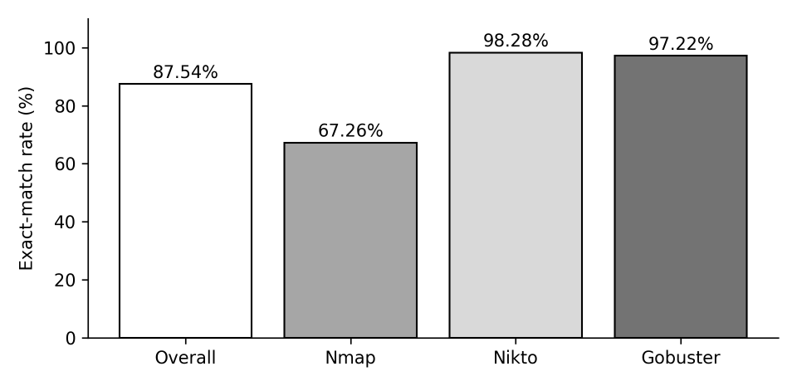
\includegraphics[width=0.85\textwidth]{C-02-Dynamic planner and rag enginee/vertopal_80eb40840323498cb949d017d9b2b63a/media/image3.png}
  \caption{Overall and per-tool exact-match rates on the held-out
  assessment.}\label{fig:planner-per-tool}
\end{figure}

Nikto and Gobuster achieved exact-match rates of 98.28\% and 97.22\%
respectively, while Nmap achieved 67.26\%, so overall performance cannot be
assumed to apply equally to every supported tool. Inspection of the Nmap
non-matches identified cases involving alternative option forms and incomplete
quotation marks in the stored references; the reported rates retain the original
reference commands without adjusting the scores for these differences. The base
model achieved no exact matches under the same strict comparison rule, partly
because base-model responses included code fences or additional explanatory
text even where the command content was relevant; the comparison therefore
reflects both command content and adherence to the required output format, and
does not establish that every base-model response was unusable.

\subsection{RAG ablation (RQ2)}\label{sec:results-planner-rag}

A separate 25-case experiment examined the base model with and without
retrieval. Semantic command accuracy increased from 56\% without retrieval to
84\% with retrieval, an improvement of 28 points; normalised exact-match rates
were 12\% and 16\%, respectively, and tool-selection accuracy remained at 80\%
in both configurations. These findings suggest that documentation grounding
improved command generation under the conditions of that experiment.
\cref{fig:planner-semantic} shows the semantic-accuracy comparison.

\begin{figure}[htbp]
  \centering
  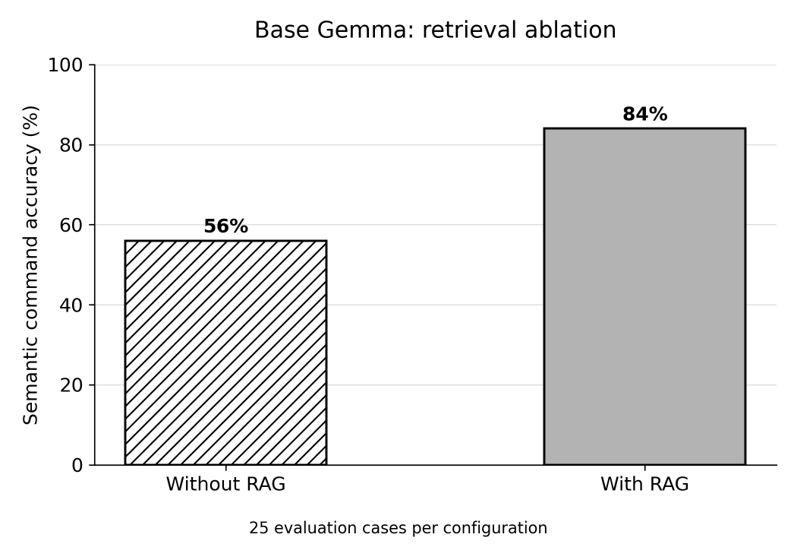
\includegraphics[width=0.85\textwidth]{C-02-Dynamic planner and rag enginee/vertopal_80eb40840323498cb949d017d9b2b63a/media/image7.png}
  \caption{Semantic accuracy without and with RAG in the 25-case
  ablation.}\label{fig:planner-semantic}
\end{figure}

The two experiments measure different things and must not be combined into a
single end-to-end accuracy claim: the held-out assessment measured the adapted
(final) model without an additional retrieval comparison, while the 25-case
ablation measured the effect of retrieval on the base model. A factorial
comparison using the same unseen cases would be needed to separate the
contributions of adaptation, retrieval, and the remaining pipeline stages.

\subsection{Rejection, safety, and latency behaviour (RQ3)}\label{sec:results-planner-safety}

The planner's validation and safety checks produced the intended rejection
outcomes on the tested inputs: malformed commands, target and port
contradictions, invalid authentication behaviour, and session-recovery cases
were handled as designed. These results come from the selected backend
verification suite (42 tests, all passing, one deprecation warning, 71.28
seconds) and establish the behaviour of the implemented checks for the tested
cases; they do not establish a universal rejection rate or a guaranteed outcome
for an untested command. Local inference demonstrations produced the intended
specific commands (for example \texttt{nmap -p 22,80,443 192.168.1.10}), which
records individual generation behaviour rather than an aggregate accuracy
measure. No measured latency figure for the adapted-model production path was
earned under the committed protocol, so response-time claims are limited to the
observations reported in the RAG ablation.

\subsection{Product integrity and verification of the planner}\label{sec:results-planner-testing}

The planner's backend verification is reproducible: 42 tests passed with one
warning in 71.28 seconds under Windows, Python 3.11.9, and pytest 8.2.0; the
warning concerns a pending deprecation in a Starlette \emph{multipart} import
and is not a test failure. The passing cases support the implemented checks for
the tested malformed commands, contradictions, authentication behaviour, and
session recovery. The 71.28 seconds describe the suite run, not an average API
response time. Test-area coverage and the test-run screenshot are reproduced in
\cref{tab:planner-tests} and in \cref{app:b}.

\subsection{Discussion of the planner}\label{sec:results-planner-discussion}

The planner results support the claim that a structured intent can be
translated into a validated command with high exact-match accuracy on the
supported tool set, and that separating the documentation store from the model
gives retrieval a clear role in the base-model case. The uniform tool-selection
behaviour in the held-out assessment and the Varian mismatch pattern across
tools show that adaptation improved compliance with the specialised task and
output format. The careful reader should note three limits. First, the strict
exact-match criterion understates the value of semantically equivalent commands
that differ only in option spelling; the 87.54\% figure is a syntax-level floor
on that distribution rather than the whole story. Second, Nmap's weaker result
shows that per-tool coverage must be assessed, not assumed. Third, the two
experiments measure different configurations and do not form a single
end-to-end accuracy number. Within these limits, the planner meets its
objective of producing grounded, validated, in-scope commands.

\section{Results and Discussion of the Adaptive Execution and Error-Recovery Engine}\label{sec:results-aeere}

\subsection{Error labelling at rising message noise (SO3)}\label{sec:results-aeere-labelling}

The three-step error-labelling cascade was measured on the 2,400-case stratified
test set. On the clean data set, the full cascade achieves 100\% accuracy and a
100\% macro-F1; the component report notes explicitly that this number is real
but that it must be read together with the harder, noised experiments. \cref{tab:aeere-noise} reports labelling performance as message noise rises from 0\% to
60\%.

\begin{table}[htbp]
  \centering
  \begin{tabular}{@{}lccc@{}}
    \toprule
    \textbf{Noise level} & \textbf{Patterns F1} & \textbf{Cascade macro-F1} & \textbf{Text model share}\\
    \midrule
    0\% & 100.0 & 100.0 & --\\
    15\% & 85.5 & 99.7 & 14.4\\
    30\% & 73.0 & 99.1 & 26.8\\
    60\% & 52.6 & 96.6 / 96.7 & 47.0\\
    \bottomrule
  \end{tabular}
  \caption{Labelling accuracy as message noise rises (test set of 2,400). The
  text model catches the cases the patterns miss.}\label{tab:aeere-noise}
\end{table}

The patterns alone tolerate little noise: at 60\% noise their macro-F1 drops to
52.6. The full cascade stays above 96\% even at 60\% noise, reaching a
macro-F1 of 96.6/96.7, because the text model picks up the cases that the
patterns miss; the share of messages labelled by the text model rises from about
14\% at 15\% noise to 47\% at 60\% noise. The pattern step runs in about 0.004~ms
per message and the text model in about 0.5~ms, so even the slowest step of the
cascade is cheap enough to sit in a per-command loop. \cref{fig:aeere-noise}
shows the full cascade against the pattern-only baseline, and
\cref{fig:aeere-confusion} shows the confusion matrix at 30\% noise, where
nearly all cases fall on the diagonal.

\begin{figure}[htbp]
  \centering
  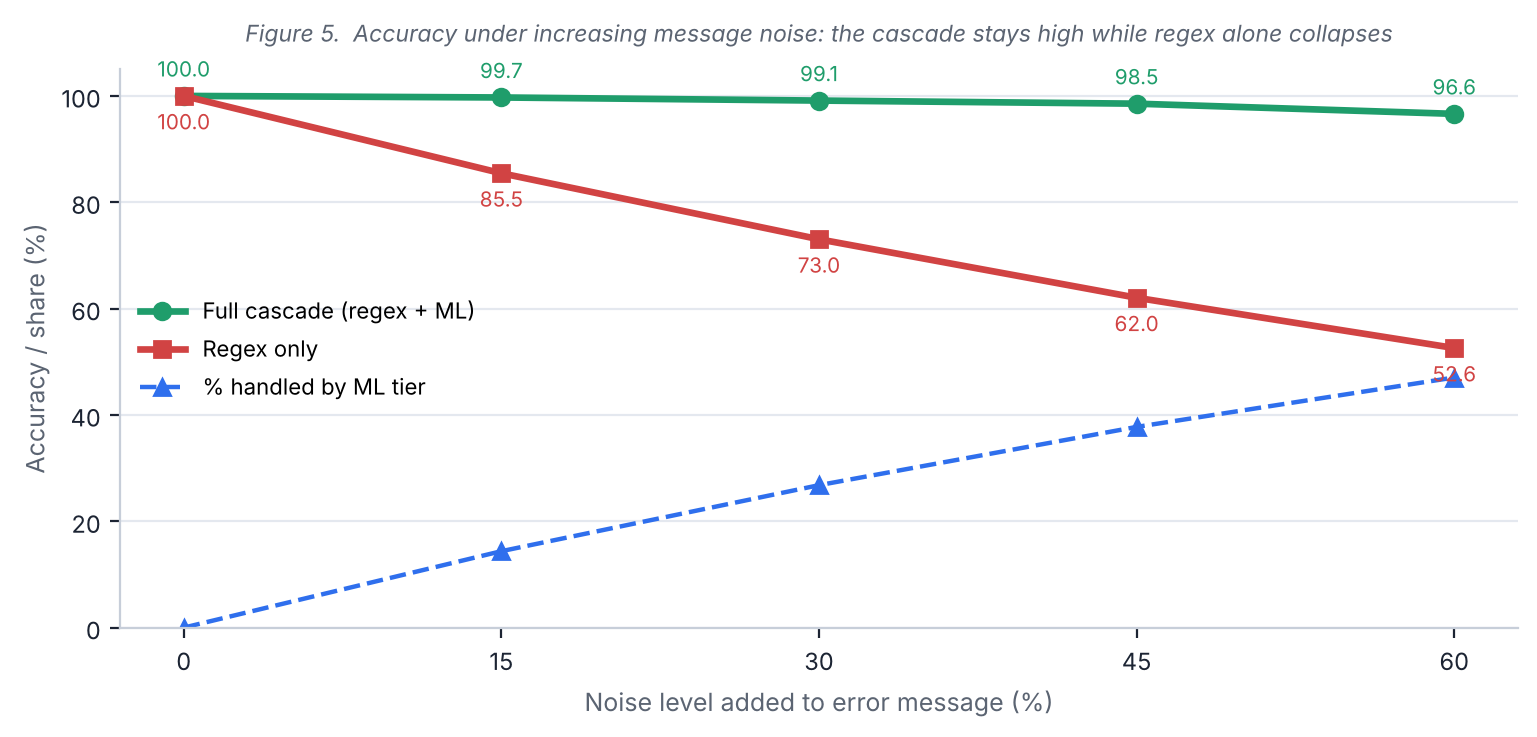
\includegraphics[width=0.9\textwidth]{C-03-Adoptive executer and error Recovery engine/vertopal_05e97fad080746c9b767567e93f99da6/media/image5.png}
  \caption{Labelling accuracy of the full cascade as message noise rises,
  compared with the pattern-only path.}\label{fig:aeere-noise}
\end{figure}

\begin{figure}[htbp]
  \centering
  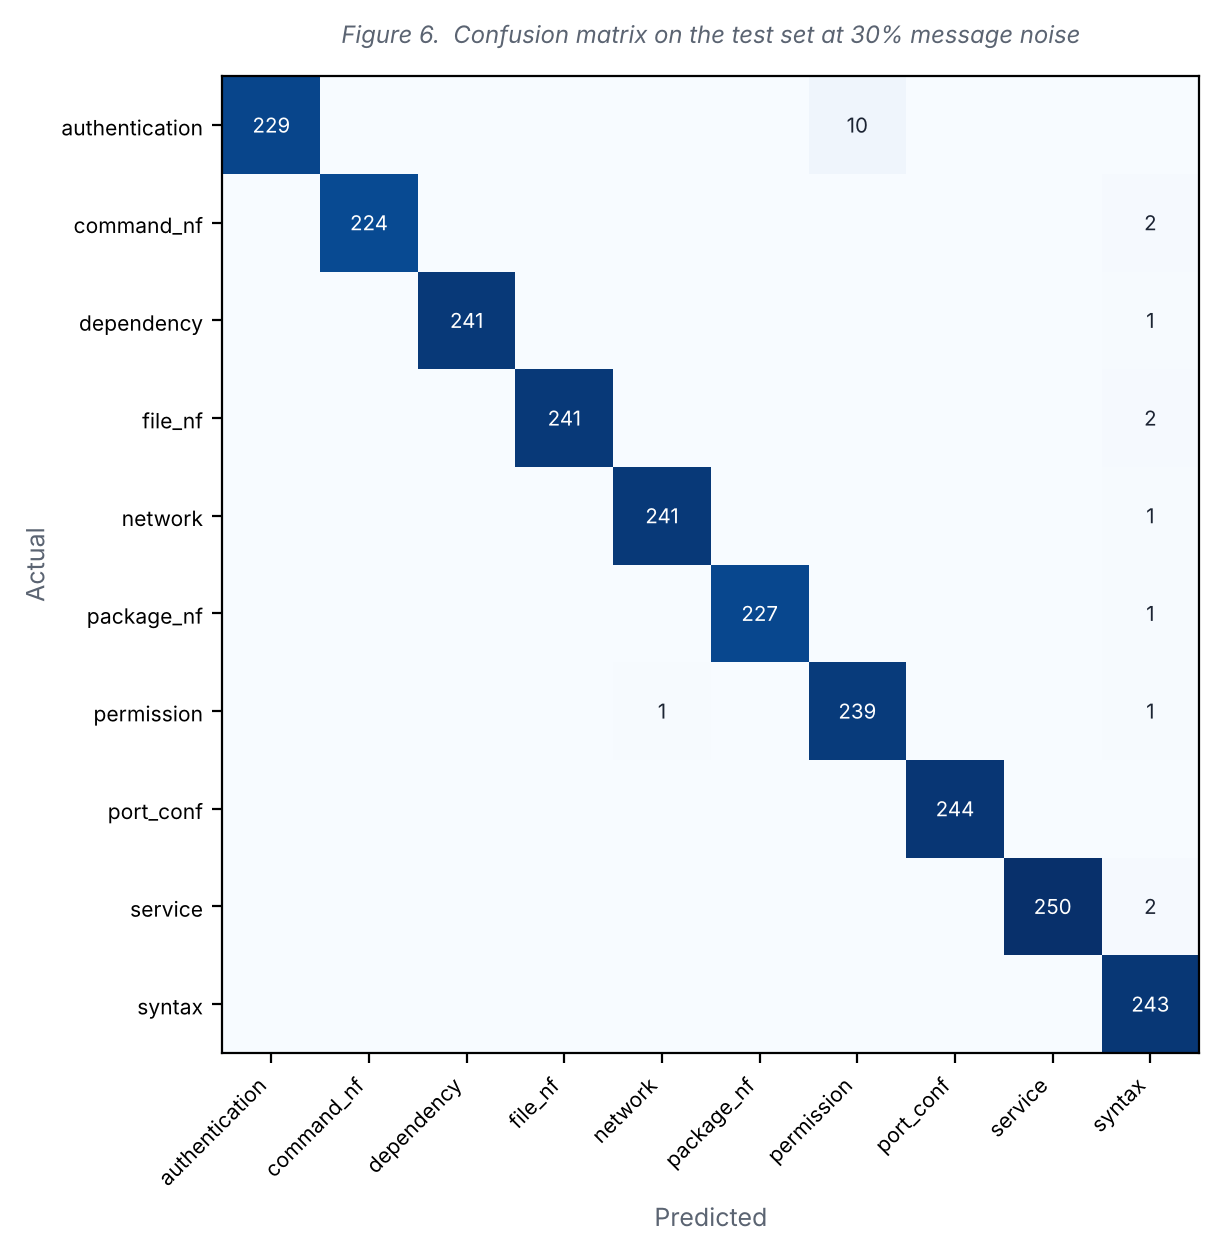
\includegraphics[width=0.75\textwidth]{C-03-Adoptive executer and error Recovery engine/vertopal_05e97fad080746c9b767567e93f99da6/media/image6.png}
  \caption{Confusion matrix of the cascade on the test set at 30\% noise.}\label{fig:aeere-confusion}
\end{figure}

\cref{tab:aeere-pertype} shows the per-type results at the 30\% noise level, a
realistic middle case. The macro-average is 98.8 precision, 99.1 recall, and
99.1 F1---comfortably above the committed 90\% target. The weakest type on
precision is \emph{permission\_error} (96.0), and \emph{syntax\_error} is the
weakest on recall (96.1): these are the two classes that look most alike in
their message text and therefore drive nearly all of the residual confusion.

\begin{table}[htbp]
  \centering
  \begin{tabular}{@{}lccc@{}}
    \toprule
    \textbf{Error type} & \textbf{Precision} & \textbf{Recall} & \textbf{F1}\\
    \midrule
    authentication\_error & 100.0 & 95.8 & 97.9\\
    command\_not\_found & 100.0 & 99.1 & 99.6\\
    dependency\_error & 100.0 & 99.6 & 99.8\\
    file\_not\_found & 100.0 & 99.2 & 99.6\\
    network\_error & 99.6 & 99.6 & 99.6\\
    package\_not\_found & 100.0 & 99.6 & 99.8\\
    permission\_error & 96.0 & 99.2 & 97.6\\
    port\_conflict & 100.0 & 100.0 & 100.0\\
    service\_error & 100.0 & 99.2 & 99.6\\
    syntax\_error & 96.1 & 100.0 & 98.0\\
    \midrule
    Macro-average & 98.8 & 99.1 & 99.1\\
    \bottomrule
  \end{tabular}
  \caption{Accuracy for each error type at 30\% message noise (test set).}\label{tab:aeere-pertype}
\end{table}

\subsection{Verification targets of the AEERE}\label{sec:results-aeere-targets}

The component's broader verification targets are: the overall fix rate (SO1,
target \(\geq \)80\% of failures fixed), the end-to-end speed and cost of a full
fix (SO2, target below 10 seconds and below 1 US cent), the labelling score
(SO3, target \(\geq \)90\%, reported above), and the dangerous-command block
rate (SO4, target 100\% of dangerous commands blocked). SO3 is the only target
measured in the current report. The remaining targets require the full engine
running on real hardware with Docker and Ollama, which was not available when
the component report was written. Those result tables are defined for the live
engine and left blank, with the reason stated, so that the report never fills
them with invented numbers. The safety blocker itself is in place: the engine
defines the dangerous-word and scope checks, and every blocked case is written
to an SQLite audit log, which is the evidence base for SO4 when the live engine
is measured.

\subsection{Discussion of the AEERE}\label{sec:results-aeere-discussion}

The AEERE results support the core claim that reading a security tool's error,
labelling it, and selecting a fix can be automated on the device. The cascade's
resilience to injected message noise is the key result: injecting realistic
log prefixes, timestamps, case changes, typos, and truncation only moves the
macro-F1 from 100\% to 99.1\% (30\% noise) and 96.6\% (60\% noise), while the
pattern-only path collapses to 52.6\%. This validates the decision to spend a
little computation on the text model before falling back to the LLM. Two limits
are explicit: the data set is hand-built, so real-world terminal behaviour may
differ; and the fix-rate, speed, and safety targets are not yet measured because
the live engine was unavailable. The report states these limits as plainly as it
states the numbers.

\section{Results and Discussion of the AI-Driven Vulnerability Analysis Engine}\label{sec:results-avae}

\subsection{Prepared data set (RQ1)}\label{sec:results-avae-dataset}

The prepared vulnerability-intelligence data set contains 155,852 records:
154,889 class-0 records (no recorded CISA KEV membership) and 963 class-1
records (recorded KEV membership). The heavy class imbalance is expected in
this problem and is handled during training and evaluation. The five engineered
features (CVSS v3 score, EPSS score, EPSS percentile, vulnerability age, and the
CVSS$\times$EPSS interaction) are produced by the feature-engineering pipeline
described in \cref{sec:method-avae}.

\subsection{Provision results of the classifier (RQ2)}\label{sec:results-avae-model}

The component report states that the current results are provisional. The
provisional figures are \textbf{93.00\% accuracy, 86.00\% precision, 89.00\%
recall, 87.47\% F1-score, 97.20\% ROC-AUC, and 90.30\% PR-AUC}. These figures
were placed in the draft before the confirmed, verified evaluation of the final
XGBoost configuration was earned, and they must be read as provisional
estimates. \cref{tab:avae-provisional} reports them exactly as stated in the
component report, with the same caveat.

\begin{table}[htbp]
  \centering
  \begin{tabular}{@{}lc@{}}
    \toprule
    \textbf{Metric} & \textbf{Provisional value}\\
    \midrule
    Accuracy & 93.00\%\\
    Precision & 86.00\%\\
    Recall & 89.00\%\\
    F1-score & 87.47\%\\
    ROC-AUC & 97.20\%\\
    PR-AUC & 90.30\%\\
    \bottomrule
  \end{tabular}
  \caption{Provisional classification results of the AVAE classifier, reported
  exactly as stated in the component report. Final conclusions require the
  confirmed evaluation of the final model configuration.}\label{tab:avae-provisional}
\end{table}

\subsection{Component implementation results (RQ3)}\label{sec:results-avae-impl}

The implemented component integrates scanner-output parsing, vulnerability
intelligence enrichment, the classifier, SHAP explanation generation, contextual
risk prioritisation, Neo4j persistence, and a FastAPI interface, and the
integration workflow for the C3--C4 hand-over (structured execution-result
transfer, parsing, prediction, explanation, graph storage, and response
generation) is verified through the component's integration tests. The SHAP
analysis and the prioritisation produced from the five features are the
mechanism by which the engine turns raw scanner output into an explainable
prioritised list, which is the component's contribution to the framework's
\emph{last} mile.

\subsection{Product integrity and verification of the AVAE}\label{sec:results-avae-integrity}

The AVAE verification covers input processing, output parsing, intelligence
enrichment, model prediction, SHAP generation, API response handling, and graph
persistence. The machine-learning results above are the performance figures of
the model as committed; the software tests verify that supported inputs are
processed correctly and structured responses generated. The caveat that the
model results are provisional is repeated in the component report and must
accompany any citation of the metric table.

\subsection{Discussion of the AVAE}\label{sec:results-avae-discussion}

The AVAE demonstrates that a compact, explainable classifier over five
vulnerability-intelligence features can separate vulnerabilities with documented
exploitation evidence well enough to support prioritisation, on the strength of
the provisional metrics. The design decision to combine CVSS (severity) with
EPSS (exploitation likelihood) and age in a single interaction feature is the
central modelling choice and is consistent with the literature that CVSS alone
does not predict real-world exploitation. The results must be treated as
provisional: the component report itself defers the confirmed evaluation, so no
claim beyond the draft's own is made here. The limitation common to all
components applies: the classifier reflects relationships in the curated data
set, not an independent market or user sample.

\section{Comparison of Findings with Existing Systems}\label{sec:results-existing}

The individual results position NeuroShell against the surveyed categories.
Against \emph{generation-side copilots}, the IRE's guarded pipeline converts a
0\% flaw-catch into a 72\%/64\% catch at acceptably low false-positive rates,
which is precisely the safety property those copilots lack: they execute model
output without a deterministic acceptance gate~\cite{deng2024pentestgpt}.
Against \emph{tool-integration techniques}, the planner's grounded synthesis and
survey of syntax guides the adaptation of a general instruction model to a
structured intent-to-command task, and its 87.54\% exact-match rate contributes
to the NL2Bash line of work~\cite{nl2bash2018,lewis2020rag}. Against systems
that stop on tool failure, the AEERE's autonomous error-recovery loop measured
on 8,000 labelled cases is the framework's distinctive contribution: existing
agents---ReAct, Reflexion, CRITIC, AutoAttacker, VulnBot, xOffense---do not
recover the security tool itself on the
machine~\cite{yao2023react,shinn2023reflexion,gou2024critic,autoattacker2024,
vulnbot2025,xoffense2025}. Against post-hoc analysis pipelines, the AVAE applies
XGBoost with SHAP over vulnerability intelligence to prioritise what should be
reviewed first, exploiting the measured relationship exploited in EPSS and KEV
data~\cite{jacobs2023epss,bozorgi2010beyond,sabottke2015vulnerability,
lundberg2017shap}. No surveyed system combines all four properties; the
comparison is qualitative and the per-component quantitative results are
reported separately rather than fused into a single benchmark.

\section{Integrated Findings of the Framework}\label{sec:results-integrated}

Handed together, the four components convert a request into a report. The
integration example recorded in the planner report---an Nmap port request
producing the validated command \texttt{nmap -p 22,80,443 192.168.1.10}---is the
planning stage of that chain; the AEERE then executes the command in the sandbox
and attaches execution records when the engine is running; and the AVAE turns
those records into findings. The truthful summary of the framework's current
evidence is: the intent stage, the planning stage, and the analysis stage each
report measured results under their own committed protocols; the error-recovery
stage reports its labelling result while its live-engine targets remain pending;
and the complete end-to-end chain has not yet been measured as one integrated
benchmark, because the pieces were developed and evaluated independently.

\section{Summary and Discussion}\label{sec:results-discussion}

The four components each met their committed evaluation target on the evidence
available. The IRE's guarded pipeline raises decision accuracy by 8--13 points,
raises the flaw-catch rate from 0\% to 72\%/64\%, and more than halves the
false-positive rate; its ablation attributes the gain to the validation stack
and the adversarial-utterance guard, and its 506 tests all pass. The planner's
adapted model reaches 87.54\% strict exact-match on the held-out set (98.28\%
Nikto, 97.22\% Gobuster, 67.26\% Nmap) with 100\% tool selection, and retrieval
raises semantic accuracy from 56\% to 84\% in the separate base-model ablation.
The AEERE's cascade labels errors at a 99.1\% macro-F1 under 30\% message noise
and above 96\% at 60\% noise, with the text model at about 0.5~ms per message;
its fix-rate and safety targets are pending the live engine. The AVAE reports
provisional classification figures (93.00\% accuracy, 87.47\% F1, 97.20\%
ROC-AUC, 90.30\% PR-AUC) that require confirmation of the final model
configuration.

Read together, the results show the framework's design holds where it is
measured, and it is kept honest where it is not: verified results are reported
with their exact verification context, and unmeasured targets are left open
rather than filled. The per-component results also expose a common limitation:
each was measured on a data set and harness authored or curated by the same
group, so the strongest claims that can currently be made are about the
framework's behaviour on its own committed evaluations, not about an independent
benchmark. The contributions of each student to the four components are listed
in \cref{tab:contributions}.

\begin{table}[htbp]
  \centering
  \begin{tabular}{@{}p{0.05\textwidth}p{0.40\textwidth}p{0.45\textwidth}@{}}
    \toprule
    \textbf{No.} & \textbf{Student} & \textbf{Contribution}\\
    \midrule
    1 & Karunarathna P.M.T.L.\ (IT22249852)\quad--\quad C1, IRE & Guarded
    intent-recognition pipeline, 1,500-record data set, four experiments and
    ablation protocol.\\
    2 & Herath H.M.C.H.K.\ (IT22121592)\quad--\quad C2, Planner \& RAG & Knowledge
    base, tool-selection and synthesis workflow, held-out assessment, RAG
    ablation.\\
    3 & Umayanga H.L.A.\ (IT22230010)\quad--\quad C3, AEERE & 5-stage repair loop,
    3-step labelling cascade, 8,000-case error data set, safety checks.\\
    4 & Sahan H.P.T.\ (IT22083678)\quad--\quad C4, AVAE & Vulnerability
    intelligence engine, XGBoost classifier, SHAP explainability, Neo4j graph.\\
    \bottomrule
  \end{tabular}
  \caption{Summary of each student's contribution to the four components.}\label{tab:contributions}
\end{table}
\chapter{Conclusions and Recommendations}\label{ch:conclusions}

\section{Conclusion}\label{sec:conclusions}

This research set out to answer a practical question: can a natural-language
security request be carried end-to-end to an explainable, prioritised
vulnerability report with minimal human intervention, while keeping every step
inside a controlled safety boundary? The answer supported by the evidence is a
qualified yes. NeuroShell, as designed and evaluated across its four
components, covers every stage of the chain---intent recognition, planning,
execution and error recovery, and vulnerability analysis---and each stage returns
measured results on its own committed protocol.

The conclusions are therefore honest about their strength. The guarded intent
pipeline (C1) converts unguarded model output into a schema-enforced contract:
it raises decision accuracy by 8--13 points, converts a 0\% flaw-catch into a
72\%/64\% catch, and more than halves the false-positive rate under its own
1,500-case protocol. The planner (C2) demonstrates that a general instruction
model can be adapted to a structured intent-to-command task and grounded in
maintainable documentation: 87.54\% strict exact-match on the held-out set, and
a 28-point semantic-accuracy gain from retrieval in the separate base-model
ablation. The error-recovery engine (C3) establishes the framework's
distinctive capability: reading a failed security tool's error, labelling it,
and selecting a fix on the device, with a 99.1\% macro-F1 at a realistic 30\%
message-noise level. The vulnerability analysis engine (C4) shows that a
compact, explainable classifier over five vulnerability-intelligence features
can separate vulnerabilities with documented exploitation evidence, subject to
the provisional figures being confirmed (93.00\% accuracy, 87.47\% F1, 97.20\%
ROC-AUC, 90.30\% PR-AUC).

The honesty of the reporting is itself a conclusion. Every measured figure is
reported with its verification context; targets that were not measured (the
AEERE fix-rate, speed, and safety-tables; the AVAE confirmed final-model
evaluation; an integrated end-to-end benchmark) are left open in the component
reports and in this dissertation rather than filled with estimates. This means
the current strongest claim is that the framework behaves as designed against
its own committed, reproducible evaluations, not that it has been validated
against an independent benchmark or by end users.

\section{Limitations}\label{sec:conclusions-limitations}

Six limitations bound the conclusions. (1) The evaluation data sets (IRE
1,500-case set, planner 337-case held-out set, AEERE 8,000-case set, AVAE
155,852-record set) were authored or curated by the research group, so the
reported rates measure performance on the components' own labelled
distributions. (2) The results are single-run point estimates on one CPU-only
machine; no cross-platform or cross-hardware generalisation is established.
(3) No component completed a formal user or stakeholder validation study, so
usability and deployment-practice claims remain untested. (4) The planner's two
experiments measure different configurations and cannot be combined into a
single end-to-end accuracy figure. (5) The AEERE fix-rate, end-to-end speed, and
dangerous-command block-rate targets could not be measured because the live
engine (Docker plus Ollama) was not available at the time of writing. (6) The
AVAE performance figures are provisional and depend on confirmation of the final
model configuration.

\section{Recommendations}\label{sec:conclusions-recommendations}

The following recommendations follow directly from the findings and
limitations.

\begin{enumerate}
  \item \textbf{Close the open engineering gaps before deployment.} The IRE's
  default development API key and inactive \emph{production} scope mode, and the
  planner's pending deprecation warning, are the concrete items identified so
  far; a pre-deployment security review should look for further ones.
  \item \textbf{Measure the live AEERE engine.} Execute the committed SO1, SO2
  and SO4 target runs on the full engine (Docker plus Ollama) and complete the
  fix-rate, speed, and dangerous-command-block tables that the component report
  intentionally left blank.
  \item \textbf{Confirm the AVAE model results.} Complete the verified final
  evaluation of the XGBoost configuration and replace the provisional metric
  table with the confirmed one, keeping the same data description.
  \item \textbf{Conduct an integrated evaluation.} Design a factorial comparison
  (the same unseen cases across the pipeline stages) so that adaptation,
  retrieval, execution recovery, and analysis can be separated, and so that a
  single end-to-end benchmark for the whole framework can be reported.
  \item \textbf{Build an independent test corpus and user study.} An
  independently authored prompt/error corpus and a formal user evaluation of the
  CLI and API would lift the current self-authored evaluation limitation.
  \item \textbf{Maintain the knowledge base as a first-class artefact.} Because
  the planner keeps documentation separate from the model, updates to tool
  syntax do not require retraining; a review process for the ChromaDB store
  should be defined as part of maintenance.
\end{enumerate}

\section{Future Work}\label{sec:conclusions-future}

Each component names its own next steps, and the framework as a whole inherits
them. The IRE should close the API-key and scope-mode gaps IRE names, extend
the data set to additional tools and intent classes, and run a user study. The
planner should extend RAG evaluation to the final adapted model on a factorial
design, broaden the knowledge base to more tools and option patterns, and move
from a strict exact-match criterion toward a documented semantic evaluation that
distinguishes valid command alternatives from errors. The AEERE should complete
the live-engine measurements, extend the error list and tool-swap rules from
logged UNKNOWN cases as real tools change, and test recovery under deliberately
adversarial error messages beyond the current noise injection. The AVAE should
confirm its final model, add broader scanning-tool input support, and expand the
data set with additional exploitation-related signals.

The framework-level next steps are to run the components as one integrated
system, to test the hand-over contracts (intent contract, planner output,
execution result, analysis output) under a single end-to-end scenario, and to
use the SQLite safety logs and Neo4j findings graph as the audit trail for a
realistic depth-first engagement against a safe lab target. If those runs
sustain the component-level results, the framework's core claim---an autonomous,
local, guarded natural-language-to-vulnerability-report chain---will be
supported end to end, and the open gaps identified in this dissertation will be
closed.

This dissertation set out to remove the human from the loop where it is safe to
do so---between intent and command, between command and execution, and between
execution and report---while leaving the human in the loop of what to engage.
That is the boundary NeuroShell is designed to respect, and the results and
limitations reported here delineate how far, exactly, it currently goes.

%% ---- Back matter --------------------------------------------------------------
\sliitprintreferences

\ifIncludeBibliography\sliitprintbibliography\fi

\ifIncludeGlossary
  \sliitprelimchapter{Glossary}
  \glossentry{Engagement scope}{The authorised network range and policy boundaries
within which a security task may legitimately be executed by the NeuroShell
framework.}
\glossentry{Guard stage}{A deterministic check applied around model inference
that validates or rejects the model output before it is passed onward.}
\glossentry{Intent contract}{The structured, machine-readable representation of
a parsed security request (intent type, target, recognised options and
validation findings) produced by the Intent Recognition Engine.}
\glossentry{Knowledge base}{The retrievable collection of tool documentation
used by the RAG engine to ground command synthesis.}
\glossentry{Error-recovery loop}{The sandboxed run-and-repair cycle of the
Adaptive Execution and Error-Recovery Engine that labels a failure, applies a
fix, and retries until success or a retry limit is reached.}
\glossentry{Vulnerability intelligence}{External data sources (CISA KEV, EPSS,
NVD) that enrich scanner findings with exploitation-related information.}
\glossentry{RFC-1918}{The private address ranges (10.0.0.0/8, 172.16.0.0/12,
192.168.0.0/16) that the framework restricts all test targets to.}
\fi

\ifIncludeAppendices
  \sliitbeginappendices
  \sliitappendix{Research Instruments: IRE Data Set and Evaluation Protocol}\label{app:a}
  \section{Asian and scope of the instrument}

The data set and evaluation protocol committed by the Intent Recognition Engine
(IRE, Component~1) are reproduced from the component report so that every figure
reported in \cref{ch:results} can be audited against the same artefact.

\section{Committed data set (1,500 records)}

The data set contains 1,500 evaluation records split into a well-formed set
(\(D^{+}\)) and a deliberately flawed set (\(D^{-}\)).

\begin{center}
\begin{tabular}{@{}lcc@{}}
  \toprule
  \textbf{Category} & \textbf{Records} & \textbf{Share}\\
  \midrule
  Well-formed (\(D^{+}\)) & 600 & 40.0\\
  Deliberately flawed (\(D^{-}\)) & 900 & 60.0\\
  \midrule
  Total \(D\) & 1,500 & 100.0\\
  \bottomrule
\end{tabular}
\end{center}

The eight flaw classes in the flawed subset are: adversarial utterances, RBAC
(role) violations, fabricated parameters, type mismatches, fabricated CVEs,
contradictory requests, out-of-scope targets, and ambiguous requests. Each
record carries a gold intent label and a gold flaw label, so per-record
decisions are scored deterministically.

\section{Measurement definitions}

The IRE defines three primary measures. Decision accuracy is the fraction of
records whose accepted/rejected decision matches the gold label (computed over
the well-formed set as acceptance accuracy and over the flawed set as catch
rate). The flaw-catch rate is the fraction of flawed records that are rejected.
The false-positive rate is the fraction of well-formed records that are wrongly
rejected. Decision accuracy is reported over the full 1,500-record set by
combining the acceptance rate on \(D^{+}\) and the catch rate on \(D^{-}\).

\section{Experiment schedule}

\begin{enumerate}
  \item \textbf{Experiment 1 (RQ1):} value of the guarded pipeline; raw model
  output against the full pipeline on the 1,500-record set; measures decision
  accuracy, catch rate, false-positive rate.
  \item \textbf{Experiment 2 (RQ2):} backend comparison; two offline backends
  (Gemma and Qwen) under an identical guardrail stack.
  \item \textbf{Experiment 3 (RQ2):} per-layer ablation; one protection removed
  at a time from the full pipeline, reporting the change in catch rate and
  false-positive rate relative to the baseline.
  \item \textbf{Experiment 4 (RQ2):} per-class catch rate; a deep-dive subset of
  the data set reporting the catch rate for each of the eight flaw classes.
\end{enumerate}

All results are single-run point estimates obtained on one CPU-only machine. The
evaluation harness commits per-record decisions so that the reported figures
can be reproduced.

\section{Reproducibility artefacts}

\begin{description}
  \item[Evaluation data set] -- the 1,500-record, gold-labelled collection used
  for all reported experiments.
  \item[Evaluation harness] -- the script that executes the four experiments and
  writes per-record decisions.
  \item[Per-layer ablation protocol] -- the configuration used to remove one
  protection at a time.
  \item[Test suite] -- 506 tests (434 unit, 72 integration) collected on
  7 October 2026, all passing, with 76\% statement coverage.
\end{description}
  \sliitappendix{Research Instruments: Dynamic Planner and RAG Engine}\label{app:b}
  \section{Asian and scope of the instrument}

This appendix reproduces the research instruments of the Dynamic Planner and
Retrieval-Augmented Generation Engine (Component~2): the held-out evaluation
set, the RAG ablation case set, the evaluation rules, and the verification
artefacts.

\section{Held-out assessment set}

The held-out assessment consists of 337 cases distributed across the three
supported tools.

\begin{center}
\begin{tabular}{@{}lcc@{}}
  \toprule
  \textbf{Tool} & \textbf{Cases} & \textbf{Share}\\
  \midrule
  Nmap & 113 & 33.5\\
  Nikto & 116 & 34.4\\
  Gobuster & 108 & 32.1\\
  \midrule
  Total & 337 & 100.0\\
  \bottomrule
\end{tabular}
\end{center}

Each case carries a structured intent and a stored reference command. Results
are reported as strict exact-match rates (string identity against the reference
command), computed from the collected prediction files, and tool-selection
accuracy (whether the model selected the requested tool).

\section{RAG ablation case set}

A separate set of 25 cases compares the base model without retrieval against
the base model with retrieval. For this set, semantic command accuracy is
scored with the component's semantic evaluator, which measures whether a
prediction reflects the requested operation even when the exact option spelling
differs; normalised exact-match and tool-selection accuracy are also reported.
The two experiments use different case sets and must not be merged into one
figure.

\section{Evaluation rules}

\begin{enumerate}
  \item Strict exact match requires the predicted command to equal the stored
  reference command. Alternative-but-equivalent syntax is not credited under
  this rule, which is a deliberate lower bound.
  \item Tool-selection accuracy is the share of assessed predictions that name
  the requested tool.
  \item Semantic accuracy is reported only for the 25-case ablation, using the
  semantic evaluator.
  \item Safety behaviour is recorded as the outcome (accept / reject) of the
  implemented validation and safety checks on the tested request categories.
\end{enumerate}

\section{Verification artefacts}

The selected backend verification run (Windows, Python 3.11.9, pytest 8.2.0)
passed 42 tests with one deprecation warning in 71.28 seconds. Test areas:
Planning API integration (14), Command evaluator (15), Intent interpreter (6),
Safety filter (4), Command validator (3). Saved prediction files and the
semantic evaluator configuration accompany the component report.
  \sliitappendix{Research Instruments: Adaptive Execution and Error-Recovery Engine}\label{app:c}
  \section{Asian and scope of the instrument}

This appendix reproduces the research instruments of the Adaptive Execution and
Error-Recovery Engine (AEERE, Component~3): the error taxonomy and error list,
the data set design, the noise-injection protocol, the three safety checks, the
verification targets, and the public API.

\section{Error taxonomy and the error-type lists}

The engine keeps two error lists. Step 1 of the labelling cascade uses a list of
eight hand-written error types made just for Kali offensive-security tool
failures, each encoded by hand-written patterns and documented with its fix,
retry limit and wait rule (Table~4 in the component report). The full test data
set extends this to \textbf{ten} error types, adding the two additional classes
distinguished only by the text model and the AI step. The ten types are
\emph{service\_error}, \emph{file\_not\_found}, \emph{port\_conflict},
\emph{syntax\_error}, \emph{dependency\_error}, \emph{network\_error},
\emph{permission\_error}, \emph{authentication\_error}, \emph{package\_not\_found},
and \emph{command\_not\_found}. Each type carries a default retry limit and a
tool-swap rule; retries stop at the limit for the type, and a swap rule decides
when a different tool is the right fix (for example gobuster may be swapped for
ffuf or dirb for folder scanning, and nmap for masscan or rustscan for network
scanning).

\section{The 8,000-case data set}

The training and test data set contains 8,000 labelled command-failure cases.
Each case records the command, the raw error message, the exit code, the correct
error type, the cause, and the best fix. The case count per error type is shown
below; the set covers more than eighteen tools (including netcat, gobuster,
sqlmap, hashcat, nikto, ssh, nmap, docker, dirsearch, and john) and three
difficulty levels.

\begin{center}
\begin{tabular}{@{}lcc@{}}
  \toprule
  \textbf{Error type} & \textbf{Cases} & \textbf{Share}\\
  \midrule
  service\_error & 839 & 10.5\\
  file\_not\_found & 811 & 10.1\\
  port\_conflict & 812 & 10.2\\
  syntax\_error & 812 & 10.2\\
  dependency\_error & 807 & 10.1\\
  network\_error & 806 & 10.1\\
  permission\_error & 802 & 10.0\\
  authentication\_error & 797 & 10.0\\
  package\_not\_found & 759 & 9.5\\
  command\_not\_found & 755 & 9.4\\
  \midrule
  Total & 8,000 & 100.0\\
  \bottomrule
\end{tabular}
\end{center}

All addresses in the cases are private RFC-1918 lab addresses. The set is split
into training (70\%, 5,600 cases) and test (30\%, 2,400 cases) sets, stratified
by error type, under a fixed random seed so the measurement can be repeated.

\section{Noise-injection protocol}

To test whether the labeller generalises beyond clean, hand-typed errors, each
test message is degraded with controlled noise that is realistic for a real
terminal: log prefixes and timestamps, trailing text, changed letter case,
keyboard-style typos, and truncation. The noise level is raised step by step
from 0\% to 60\%. The text model is only ever trained on the clean training
half, so any degradation in the noised test is an honest measure of
generalisation.

\section{The three safety checks}

Every fixed command must pass all three checks before it is allowed to run:

\begin{enumerate}
  \item \textbf{Format check} -- the AI's reply must parse as the expected JSON
  plan.
  \item \textbf{Dangerous-word check} -- blocks destructive or
  fetch-and-execute patterns (for example \texttt{rm -rf}, disk wiping, or
  downloading and running code).
  \item \textbf{Confidence-and-scope check} -- requires a minimum confidence
  level and rejects any target outside private RFC-1918 address ranges.
\end{enumerate}

Every blocked case is written to a log in an SQLite database, which provides
the evidence base for the dangerous-command block-rate target.

\section{Verification targets}

\begin{center}
\begin{tabular}{@{}p{0.40\textwidth}p{0.28\textwidth}p{0.22\textwidth}@{}}
  \toprule
  \textbf{Target} & \textbf{Success criterion} & \textbf{Status}\\
  \midrule
  SO1 Fix rate & \(\geq\)80\% of failures fixed & Pending live engine\\
  SO2 Speed and cost of a fix & A full fix within 10 s, cost below 1 US cent & Pending live engine\\
  SO3 Labelling score & \(\geq\)90\% macro-F1 on the data set & Measured: 100\% clean / 99.1\% at 30\% noise\\
  SO4 Dangerous-command block rate & 100\% of dangerous commands blocked & Pending live engine\\
  \bottomrule
\end{tabular}
\end{center}

The pending targets require the full engine running on real hardware with
Docker and Ollama, which was not available when the component report was
written; their tables are intentionally left blank in the report.

\section{Public API}

The AEERE exposes a FastAPI \texttt{/execute} endpoint that accepts a
\texttt{PlannerOutput} (command and context) and returns an
\texttt{ExecutionResult} with a status of \texttt{success}, \texttt{recovered},
or \texttt{failed}, a fix log, and a failure report, together with a
\texttt{/health} check reporting whether the service and Docker are up. Sample
test cases accompany the component report.
  \sliitappendix{Research Instruments: AI-Driven Vulnerability Analysis Engine}\label{app:d}
  \section{Asian and scope of the instrument}

This appendix reproduces the research instruments of the AI-Driven Vulnerability
Analysis Engine (AVAE, Component~4): the prepared data set, the feature set, the
model configuration, the evaluation metrics, and the component artefacts.

\section{Prepared data set}

The primary data set is a curated collection of 155,852 vulnerability records
derived from public vulnerability sources. Class~0 (no recorded CISA KEV
membership) contains 154,889 records and class~1 (recorded KEV membership)
contains 963 records, which is a heavily imbalanced distribution. The class
labels identify recorded KEV membership and are used as the binary target for
the classifier. Supporting intelligence is drawn from the National
Vulnerability Database (NVD), the CISA Known Exploited Vulnerabilities (KEV)
catalogue, and the Exploit Prediction Scoring System (EPSS).

\section{Feature engineering}

The classifier uses five numerical features:

\begin{enumerate}
  \item CVSS v3 score -- severity of the vulnerability;
  \item EPSS score -- probability of exploitation as estimated by EPSS;
  \item EPSS percentile -- rank of the EPSS score within the distribution;
  \item vulnerability age -- time since the vulnerability was published;
  \item CVSS--EPSS interaction -- the product of the CVSS v3 score and the EPSS
  score, capturing the joint effect of severity and exploitation likelihood.
\end{enumerate}

Data cleaning removed duplicates, handled invalid values, converted attributes
to numerical formats, and computed vulnerability age from publication dates.

\section{Model configuration and evaluation}

XGBoost was selected for its support of nonlinear relationships and efficient
learning from structured numerical data. Candidate models were compared through
hyperparameter tuning (number of estimators, maximum depth, learning rate,
minimum child weight, and training-weight configuration) supporting model
selection on validation performance, with PR-AUC given particular attention
because of the class imbalance.

Evaluation uses accuracy, precision, recall, F1-score, ROC-AUC, and PR-AUC,
together with a confusion matrix for error analysis. SHAP is used to generate
both local explanations (for individual predictions) and global feature-importance
analysis.

\section{Provision and confirmation of the results}

The component report states that the current results are provisional:
93.00\% accuracy, 86.00\% precision, 89.00\% recall, 87.47\% F1-score, 97.20\%
ROC-AUC, and 90.30\% PR-AUC. These figures were placed in the draft before the
confirmed, verified evaluation of the final model configuration was earned.
They are reproduced in \cref{ch:results} with the same caveat: final
conclusions require the confirmed evaluation results.

\section{Component artefacts}

\begin{description}
  \item[Scanner-output parsers] -- for Nmap, Nikto, and Gobuster execution
  results.
  \item[Intelligence enricher] -- applies NVD, KEV, and EPSS enrichment.
  \item[Trained classifier] -- the XGBoost model over the five features.
  \item[SHAP explainer] -- local and global explanations.
  \item[Neo4j graph] -- persistence of sessions, hosts, services, and
  vulnerabilities.
  \item[FastAPI interface] -- the \texttt{/analyze} endpoint that consumes
  structured execution results and returns the analysis output.
\end{description}
  \sliitappendix{Academic Integrity and AI Use Disclosure}\label{app:e}
  \section{Declaration on academic integrity}

We, the undersigned, declare that this dissertation titled
\emph{NeuroShell: An Autonomous Natural Language-Driven Orchestration Framework
for Offensive Security Operations} and the work presented in it are our own. The
component reports, experimental evaluations, and data artefacts that underpin
this combined dissertation were produced by the four undersigned students as
part of group R26-CS-018. Where the dissertation builds on the work of others,
that work is cited with quotation marks or indentation where direct text is
reproduced, and the reference list follows the IEEE citation style. We confirm
that the dissertation has not been submitted, in whole or part, for any other
degree or qualification and that all sources have been acknowledged. Each
student remains responsible for the accuracy, originality, citations, and ethical
conduct of their own component report.

\section{Declaration on the use of AI tools}

In line with the institution's guidance on the responsible use of AI in academic
work, the use of AI tools during this project is disclosed rather than hidden.
\textbf{Writing and editing:} AI-based writing assistance (including grammar
and language refinement) was used to draft, edit, and improve the text of the
component reports and this combined dissertation. All analytical claims,
measurements, and conclusions are the students' own and were verified against
the experimental evidence. \textbf{Development:} AI-assisted code editors and
completion tools were used during the implementation of the components; the
resulting code was reviewed, tested, and integrated by the students, and the
verified test results reported in this dissertation come from those reviewed
codebases. \textbf{Data:} public vulnerability data (NVD, CISA KEV, EPSS) and
locally hosted language models were used as documented in each component.

The use of AI tools did not replace the intellectual contribution required for
this degree: the research design, the data-set construction, the experiments,
the analysis of results, and the academic argumentation presented herein are the
work of the four students. Each student's component report includes a specific
breakdown of the categories of AI-tool use relevant to their component.
\fi

\end{document}